\chapter{XChange: Generic Asset Trading in Resource-constrained Environments}
\label{chapter:xchange}

\emph{An increasing number of industries rely on Internet-of-Things devices to track physical resources.
	Blockchain technology provides primitives to represent these resources as digital assets on a secure distributed ledger.
	Due to the proliferation of blockchain-based assets, there is an increasing need for a generic mechanism to trade assets between isolated platforms.
	To date, there is no such mechanism without reliance on a trusted third party. }
	
\emph{In this work, we address this shortcoming and present XChange.
	%Unlike existing approaches for decentralized asset trading, we decouple trade management and the actual exchange of assets.
	XChange mediates trade of \emph{any} digital asset between isolated blockchain platforms while limiting the fraud conducted by adversarial parties.
	We first describe a generic, five-phase trading protocol that establishes and executes trade between individuals.
	This protocol accounts full trade specifications on a separate blockchain.
	%We show with a theoretical analysis that the effectiveness of fraud conducted by adversarial parties is limited.
	We then devise a lightweight system architecture, composed of all required components for a generic asset marketplace.}
	
\emph{We implement XChange and conduct real-world experimentation.
	We leverage an existing, lightweight blockchain, TrustChain, to account all orders and full trade specifications.
	By deploying XChange on multiple low-resource devices, we show that a full trade completes within half a second.
	To quantify the scalability of our mechanism, we conduct further experiments on our compute cluster.
	We conclude that the throughput of XChange, in terms of trades per second, scales linearly with the system load.
	Furthermore, we find that XChange exhibits superior throughput and order fulfil latency compared to related decentralized exchanges, BitShares and Waves. }

\newpage

\section{Introduction}
Bitcoin, introduced in 2008, has revolutionized the field of digital currencies by demonstrating that it is possible to devise a secure cash system without a bank~\cite{nakamoto2008bitcoin}.
The goal of Bitcoin is to realize a payment system through the secure management of a native currency on a distributed ledger.
The creation of this currency is controlled by miners participating in a voluntary process known as mining.
The collective efforts of miners ensure the security of Bitcoin and prevent illegitimate coin creation.
Miners invest computational power to include valid transactions on the blockchain, which is a tamper-proof distributed ledger that consists of blocks.
One of the compelling features of a blockchain is the ability to securely record and validate user-issued transactions without trusted intermediary, even in the presence of mutual distrust between participants.

Participation in many deployed blockchains is open for everyone and does not require the explicit approval from authorities unlike traditional banking systems.
Even though blockchain technology provides the means to maintain a distributed ledger without trusted intermediaries, open enrollment is not required for many industrial use cases, or is even undesirable.
For instance, when two companies leverage blockchain technology to securely record their transactions, read and write access to the distributed ledger is most likely limited to a few selected employees or operators.
Over the past few years, there has been a sharp increase in the development and deployment of private, or \emph{permissioned} blockchains~\cite{androulaki2018hyperledger,de2018pbft,vukolic2017rethinking}.
In contrast to a public blockchain like Bitcoin, membership in a permissioned blockchain is managed by an authority that approves the participation of each peer.
The identity under which a peer operates is linked to a real-world persona, which reduces the likelihood of Byzantine behavior and network threats like the Sybil Attack~\cite{douceur2002sybil}.
Permissioned blockchains usually adopt a classical consensus model designed for networks with static membership, e.g., Practical Byzantine Fault Tolerance (PBFT)~\cite{castro1999practical}.
Considerable efforts in permissioned blockchains have been made by projects such as Hyperledger Fabric~\cite{androulaki2018hyperledger}, R3 Corda~\cite{brown2016introducing}, Quorum~\cite{mogan2018quorum} and BigchainDB~\cite{mcconaghy2016bigchaindb}.
Permissioned blockchains have the potential to increase the efficiency of traditional business processes in industries like logistics, energy management and trade supply chains~\cite{vukolic2017rethinking}.

Several use cases that record transactions on a permissioned blockchain revolve around the representation and management of real-world assets on a distributed ledger~\cite{hewett2019inclusive}.
Advancements in blockchain technology have resulted in numerous platforms on which companies can issue and manage digital assets.
There currently is a proliferation of different types of assets, fragmented across many different blockchain implementations~\cite{borkowski2018towards}.
In public blockchains, almost 200\,000 different assets are being managed on the Ethereum blockchain only.\footnote{See https://etherscan.io/tokens}
A recent Forbes report reveals that at least 50 major companies, each valued at least at \$1 billion, are exploring blockchain technology for asset management and trading~\cite{forbes50companies}.
As industry's adoption of blockchain technology is increasing, a similar asset proliferation will occur with permissioned blockchains.
Unfortunately, there is no \emph{universal} mechanism to exchange (trade) assets between isolated distributed ledgers without the involvement of a trusted third party.
Research and developments in distributed ledger technology mostly focus on the deployment of new domain-specific blockchains, whereas interoperability issues are mostly ignored~\cite{schulte2019towards,yli2016current}.
In particular, there is a lack of research on the interoperability of permissioned, industry-grade blockchains~\cite{nikander2019interledger,vo2018internet}.
Interoperability concerns are particularly relevant when leveraging distributed ledgers for trading, as a single trade consignment can involve various isolated blockchains~\cite{ganne2018can}.
Given the inevitable growth of permissioned blockchain platforms, we argue that a universal mechanism for asset exchange between these platforms is a growing necessity.

\begin{figure}[t]
	\centering
	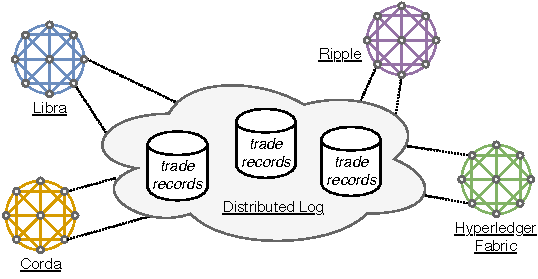
\includegraphics[width=.75\linewidth]{xchange/assets/xchange_interoperability}
	\caption{XChange coordinates the asset exchange between permissioned blockchains by storing trade records in a distributed log. This enables traders to detect if a party has committed fraud during an ongoing trade.}
	\label{fig:xchange_interoperability}
\end{figure}

We present \emph{\ModelName{}}, a universal mechanism for asset exchange, or \emph{trade}, between permissioned blockchains.\footnote{We use the terms \enquote{exchange} and \enquote{trade} interchangeably in this work.}
\ModelName{} coordinates trade between separate permissioned blockchains by storing trade records in a distributed log, also see Figure~\ref{fig:xchange_interoperability}.
Our solution is independent of the technical characteristics of the involved blockchains and does not require modifications to blockchain applications that are already operational.
An asset exchange in \ModelName{} proceeds through a sequence of alternating, unilateral asset transfer operations (payments) between two parties.
This is comparable to how many electronic markets (e.g., eBay) operate, where a party only initiates a payment back to the counterparty after having received a payment first.
Sequential payments, however, introduce a risk of losing economic value to the other party, since the other party is now able to \enquote{steal} assets during a trade~\cite{koens2019assessing}.
This fraud is called \emph{counterparty fraud} and is a severe concern in many electronic marketplaces that facilitate peer-to-peer trading~\cite{peters2016understanding}.
For this reason, we argue that any asset trading mechanism must either prevent counterparty fraud or punish a participant that has committed this fraud upon its detection.

To address counterparty fraud, existing solutions for asset exchange between distinct blockchains often provide atomic guarantees.
Atomicity in this context implies that a trade either exchanges all assets between involved parties or exchanges nothing.
We find that the security of existing solutions either (1) relies on one or more trusted intermediaries to ensure that assets are securely exchanged, or (2) relies on the availability of specialized transactions by the blockchains that manage the assets being traded.
Relying on trusted intermediaries to exchange assets is the foremost approach when trading assets on public blockchains, e.g., by using the services of a cryptocurrency exchange.
In a permissioned setting, however, this approach requires the participation of these intermediaries in the involved blockchains, which is not always allowed by their network operators.
Solutions for asset exchange that depend on specialized transactions, e.g., atomic swaps, are not universal enough to support trade between any pair of permissioned blockchains.
For example, Hyperledger Fabric does not provide support for atomic swaps by default, thus requiring modifications to deployed and operational applications.

In contrast to existing solutions, \ModelName{} particularly focuses on \emph{detection} of counterparty fraud.
We argue that the detection of counterparty fraud during a trade is sufficient, since misbehavior can always be traced back to a real-world identity, and optionally punished by an external authority.
To detect counterparty fraud, \ModelName{} requires traders to append tamper-proof trade records to a distributed log.
By recording the initiation of each trade, conducted payments, and the completion of a trade, participants can detect if a malicious trader has committed fraud and then refrain from trading with that party.

\ModelName{} does not provide atomic trade guarantees; however, it limits the economic gains of adversarial parties by introducing two risk mitigation strategies.
First, \ModelName{} allows a trade to gradually complete through multiple, smaller payments.
This is also called \emph{incremental settlement}.
With incremental settlement, traders themselves decide how much risk they are willing to take, and specify how much economic value they put at stake.
Our second risk mitigation strategy is to restrict traders that could have committed fraud during an ongoing trade, from engaging in another trade.
\ModelName{} forces an adversarial party to finish an ongoing trade first before it can trade with other parties.
We prove that this strategy effectively limits the economic gains of adversaries.
Since \ModelName{} assumes static membership through well-defined identities, it prevents a situation where a participant that has committed counterparty fraud can re-joins the network under a new digital identity and commit fraud again (the whitewashing attack)~\cite{feldman2006free}.

In this work, we first outline how existing mechanisms for cross-chain asset exchange work.
We then present our solution and describe the \ModelName{} protocol.
We deploy \ModelName{} using a tamper-proof, distributed log with low overhead, a technology that pre-dates Bitcoin~\cite{haeberlen2007peerreview}.
We leverage an existing solution, TrustChain, built for secure logging and accounting of generic data records~\cite{otte2017trustchain}.
By conducting a trade between two Raspberry Pis, we quantify that the added latency by \ModelName{} is only 493 milliseconds.
Additional experiments on our compute cluster reveal that \ModelName{} achieves over 1\,000 trades per second and that its throughput scales linearly with the system load.

%The fundamental design principle of \ModelName{} is to \emph{decouple trade management and the exchange of assets between traders}.
%The key design principle of \ModelName{} is to \emph{decouple order management and asset management}.
%Our approach is visualized in Figure~\ref{fig:idea} and originates from the observation that existing blockchain-based marketplaces for asset trading utilize the same underlying data structure to manage trade and to exchange assets.\todo{remove/rewrite?}
%Therefore, trade management is subject to the same security requirements as the exchange of assets between trading parties.
%By decoupling these two practices, we increase overall market throughput, since trade management requires different (lower) security guarantees than the exchange of assets.
%Peers in the \ModelName{} network maintain a distributed ledger that stores all orders and trade activity.
%These peers interact with external platforms to transfer assets to other traders.
%To store market activity , we build on a scalable blockchain ledger that is optimised for data accounting.
%By accounting full trade specifications, we show that the effectiveness of fraud conducted by adversarial parties is limited.

The main contribution of this work is four-fold:
\begin{enumerate}
	\item The \ModelName{} \emph{trading protocol} which specifies how assets are exchanged between permissioned blockchains by storing trade records in a distributed log (Section~\ref{sec:protocol}).
	\item \emph{Anti-fraud measures} that limit the economic gains of adversaries committing counterparty fraud.
	\item Improvements of TrustChain, a tamper-proof, distributed log used by \ModelName{}. Our improvements enables concurrent transactions and increase scalability (Section~\ref{sec:blockchain_accounting}).
	\item A functional, open source \emph{implementation} of the \ModelName{} trading protocol (Section \ref{sec:implementation}).
	\item \emph{Experimentation} around the resource usage and scalability of \ModelName{}, conducted on multiple low-resource devices and our compute cluster (Section~\ref{sec:exp_trading_low_devices} and \ref{subsec:scalability_experiment}).
\end{enumerate}

\section{Related Work and Problem Description}
\label{sec:background_problem_description}
Achieving interoperability between blockchains is a challenging problem and remains largely unsolved~\cite{zamyatin2019sok,vo2018internet,buterin2016chain}.
Most research in this direction considers cross-chain interactions between permissionless blockchains~\cite{koens2019assessing}.
There is only few research on how to achieve interoperability between permissioned blockchains, even though this is also a concern in private environments.
We first discuss existing solutions that address asset exchange between different blockchains, ranging from approaches that rely on a trusted intermediary to trust-less trading mechanisms using specialized transactions or intermediate blockchains.
Based on our findings, we then formulate the requirements for our asset exchange mechanism.

\subsection{Trusted Intermediaries}
A common approach to exchange blockchain-based assets is by using the services of a trusted intermediary.
A trade using a trusted intermediary completes as follows: two parties that agree on a trade transfer the assets for sale to one of the wallets owned by the trusted intermediary.
When this intermediary has received both assets, it finishes the exchange by transferring the appropriate assets to the other party.
In this approach, the trusted intermediary holds (temporary) ownership of the assets to be traded.
Relying on a trusted intermediary removes counterparty risk for the trading parties, but it requires both parties to have faith that the intermediary does not default or compromise their assets.

Trade through a trusted intermediary can facilitate value exchange between an extensive range of different blockchains, as long as the intermediary maintains wallets on the involved blockchains and can issue transactions in these systems to transfer the assets.
This is usually not an issue in permissionless blockchains since anyone can create accounts or wallets by generating a new cryptographic key pair.
Centralized cryptocurrency exchanges often facilitate asset trading across numerous permissionless blockchains.
Some cryptocurrency exchanges process transactions worth millions of dollars in total daily.\footnote{See https://coinmarketcap.com/rankings/exchanges}
In a permissioned blockchain environment, however, a trusted intermediary coordinating an asset exchange requires explicit approval from the operator to read and write transactions on the involved distributed ledgers.
Allowing new parties in a permissioned blockchain might be undesirable by operators since it introduces additional legal and operational risks.

\begin{figure}[t]
	\centering
	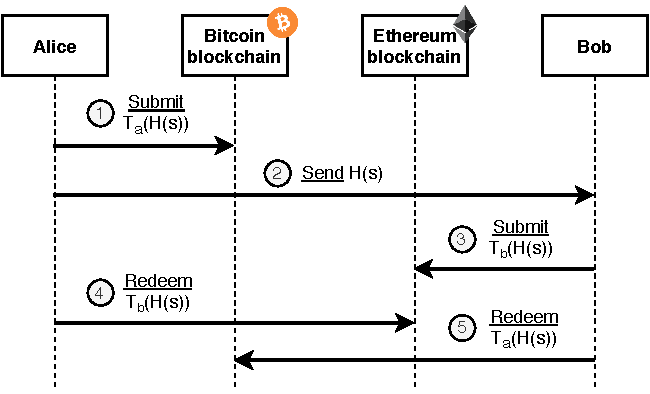
\includegraphics[width=.6\linewidth]{xchange/assets/atomic_swap}
	\caption{Sequence diagram of a successful HTLC-based atomic swap between Alice and Bob.}
	\label{fig:atomic_swap}
\end{figure}

\subsection{Atomic Swaps}
The \emph{atomic swap} is a distributed coordination task that allows asset exchange between different blockchains, without need for a trusted intermediary~\cite{herlihy2018atomic}.
Atomic swaps enable two parties to exchange blockchain-based assets with atomic guarantees: the asset exchange either completes or fails for both parties at any given time.
We now explain the involved operations during an atomic swap between the public Bitcoin and Ethereum blockchains.
Figure~\ref{fig:atomic_swap} visualizes the steps of an atomic swap between Alice and Bob, where Alice sells her Bitcoin in return for Ether (the native token of the Ethereum blockchain).
First, Alice generates a random secret $ s $ and computes $ H(s) $, where $ H(\cdot) $ denotes a hash function.
She then submits a hash-locked transaction, indicated by $ T_a(H(s)) $ (step \circled{1}), to the Bitcoin blockchain that transfers her Bitcoin to Bob's wallet address.
A hash-locked transaction is only executed when the secret $ s $ is provided to it.
Alice now sends $ H(s) $ to Bob (step \circled{2}).
Bob then submits a transaction $ T_b(H(s)) $ with the same hash lock to the Ethereum blockchain, transferring his Ethereum to the account of Alice (step \circled{3}).
Alice is now able to claim the assets held in custody by $ T_b(H(s)) $ (since she knows the value of $ s $), which in turn reveals $ s $ to Bob (step \circled{4}).
Bob now completes the swap by submitting $ s $ to the $ T_a(H(s)) $ transaction on the Bitcoin blockchain, which unlocks the assets in $ T_a(H(s)) $ (step \circled{5}).
To prevent the situation where assets are locked indefinitely if Alice refuses to reveal $ s $, Alice and Bob submit two additional time-locked transactions to ensure that assets in $ T_a(H(s)) $, respectively $ T_b(H(s)) $, can be claimed after some time $ t_1 $, respectively $ t_2 $.
To address the situation where Alice claims the assets in both $ T_a(H(s)) $ and $ T_b(H(s)) $, it must hold that $ t_1 > t_2 $.
These hash- and time-based agreements, also called Hashed Timelock Contracts (HTLCs), thus ensure trust-less, atomic asset exchange between trading parties, assuming that they claim the assets before the time-lock expires.
Atomic swaps eliminate the risk of losing assets to an adversarial trader while trading.
The HTLC atomic swap requires a total of four transactions.

Although atomic swaps enable cross-chain asset exchange, we identify a deficiency that limits their usability.
Namely, atomic swaps only work when trading assets between distributed ledgers with support for specific programming constructs, such as time-locked and hash-locked transactions.
Hyperledger Fabric, for example, requires custom application logic to support atomic swaps.
An atomic swap involving a blockchain platform without support for these transactions is not possible.
Alternative atomic swap implementations rely on smart contract execution or the availability of multi-signature transactions~\cite{zie2019extending}.

\subsection{Notary Schemes}
\label{sec:notary_schemes}
Notary schemes are another solution for asset exchange where approval by a group of credible nodes (notaries) is required to perform some operation.
Notary schemes aim to partially alleviate the trust issues arising when relying on a single trusted intermediary through the approval by a group of semi-trusted notaries instead.
These notaries reach consensus on the occurrence of particular events, e.g., on the inclusion of a transaction on a distributed ledger.
Compared to an asset exchange through a trusted intermediary, notary schemes assume a weaker trust model and can often withstand adversarial behavior of a fraction of the notaries.

The Interledger project, introduced by Ripple, is the most advanced approach in this direction~\cite{thomas2015protocol}.
Interledger proposes a notary-based protocol to conduct payments across different ledgers.
In atomic mode, these payments are realized through atomic swaps and are coordinated by a different group of notaries for every involved blockchain.
Interledger uses payment paths where additional intermediate platforms and their notaries are used to exchange assets between ledgers that do not have a direct connection.
Interledger also supports bidirectional asset exchange but is vulnerable to a fraction of notaries colluding with one of the trading parties.
External coordination is avoided in universal mode, which relies on incentives for participants to behave honestly and not to commit fraud.
The Hyperledger Quilt project provides a Java implementation of the Interledger protocol for permissioned blockchains~\cite{hyperledgerquilt}.

%We argue that notary schemes work well when exchanging assets between permissioned blockchains.
%Specifically, the entities that are managing the permissioned blockchain are suitable to take on the role as notary so no involvement of new parties is required.

\subsection{Blockchain Bridges}
Another approach to cross-chain trade uses bridging techniques, where an intermediate blockchain mediates asset exchange between different blockchains.
Most bridging approaches execute the atomic swap protocol for the exchange process of assets but provide additional primitives and interoperability features for communication between blockchains.

Blocknet is a platform for inter-blockchain routing and facilitates the exchange of cryptocurrencies between blockchains~\cite{culwick2019blocknet}.
Blocknet consists of two main components: XBridge and XRouter.
XBridge is a decentralized protocol that coordinates atomic swaps between permissioned and unpermissioned blockchains.
XRouter provides a peer-to-peer overlay network consisting of clients running the SPV protocol, therefore avoiding the need to download the full blockchain to verify the inclusion of particular transactions.
Blocknet secures its transactions through a Proof-of-Stake consensus protocol.
Furthermore, Blocknet provides a decentralized exchange where traders can indicate their trade interests through orders.
A blockchain connected to Blocknet requires the implementation of time-locked transactions.

ARK is a platform for cross-chain asset exchange that shares similarities with Blocknet~\cite{ark2019whitepaper}.
ARK enables users to build custom blockchains (a \enquote{BridgeChain}) that is powered by the ARK blockchain.
To facilitate asset exchange between different blockchains, ARK acts as an intermediate blockchain in the trade process.
The latter is achieved through the smart bridge protocol, relying on atomic swaps to exchange value across chains.
The ARK blockchain achieves transaction security through a Delegated Proof-of-Stake (dPos) consensus algorithm, where stakeholders vote for a small committee that appends blocks to the ARK blockchain.

The Proof-of-Authority (POA) blockchain is an Ethereum-based permissioned blockchain that provides several tools for interoperability~\cite{poa2018whitepaper}.
The POA blockchain is secured by the Proof-of-Authority consensus mechanism, where validating nodes stake their reputation to secure the blockchain.
The TokenBridge protocol enables users to not only exchanges assets between Ethereum-based platforms, but also facilitates arbitrary data transfer.

\subsection{Sidechains}
Sidechains provide the means to exchange assets between blockchains that share similarities, e.g., that run a particular consensus algorithm~\cite{back2014enabling}.
In essence, a sidechain is a blockchain that is attached to a parent chain.
With a two-way pegged sidechain, assets residing on the parent chain can securely be moved to the sidechain and vice versa.
These transfers lock the assets on one chain and re-create them on the connected sidechain or parent chain.
A related scheme is federated pegged sidechains~\cite{dilley2016strong}.
In a federated pegged sidechains, assets moving to another chain are controlled by a group of notaries, making this approach similar to the Interledger protocol.
Liquid is a deployed sidechain to the Bitcoin blockchain and can be used to quickly trade Bitcoin-derived currencies~\cite{dilley2016strong}.
The applicability of two-way pegged sidechains is somewhat limited since the sidechain and parent chain need to run a similar consensus algorithm.

\subsection{Internet-of-Blockchains}
Finally, we describe two solutions that aim to devise an \enquote{Internet-of-Blockchains}, where a single blockchain controls many sub-chains.
The Cosmos project, introduced by the Interchain Foundation, builds a network of heterogeneous blockchains that can seamlessly interact with each other~\cite{cosmoswhitepaper}.
The Cosmos Hub is the leading blockchain that connects many other blockchains, called zones.
Each zone can have its own governance rules and is secured using the Tendermint BFT consensus protocol.
Tokens can quickly be exchanged between the Hub and zones using the Inter-Blockchain Communication (IBC) protocol.
To interact with blockchains external to Cosmos, there is a particular zone, called a \emph{bridging zone}.
The bridging zone keeps track of transactions and blocks persisted on external blockchains, e.g., Ethereum.

The system architecture of Polkadot, introduced by Gavin Wood, is similar to Cosmos~\cite{wood2016polkadot}.
Polkadot introduces a single relay chain that is responsible for the coordination of one or more parachains.
Polkadot secures its chains through a custom consensus algorithm, inspired by Tendermint~\cite{kwon2014tendermint} and HoneyBadger~\cite{miller2016honey}.
Compared to Cosmos, Polkadot aims for a more generic message-passing algorithm between parachains that can not only transfer value.

Both Cosmos and Polkadot can facilitate the effortless exchange of assets between zones or parachains.
However, they have limited capabilities for interaction with external blockchains.
To benefit from the advantages that Cosmos and Polkadot provide, all involved companies must agree on developing their applications on the same blockchain platform, which is hard to achieve in practice.
Therefore, the advantage of Internet-of-Blockchains is questionable for industrial use cases, and a less restricting approach might be preferred when trading assets.

\begin{table}[t]
	\centering
	\begin{threeparttable}
		\begin{tabular}{ c c c c c c } 
			\hline
			\textbf{Approach} & \textbf{Universal?} & \textbf{Avoids trusted parties?} & \textbf{Guarantees atomic exchange?} \\
			Trusted Intermediary & \greencheck & \redcross & \redcross \\
			Atomic Swaps & \redcross & \greencheck & \greencheck\tnote{1} \\
			Notary Schemes & \greencheck & \redcross & \redcross \\
			Bridging & \redcross & \greencheck & \redcross \\
			Sidechains & \redcross & \greencheck & \greencheck \\
			Internet-of-Blockchains & \redcross & \greencheck & \greencheck \\ \hline
			\textbf{\ModelName{} (this work)} & \greencheck & \greencheck & \redcross\tnote{2} \\
			\hline
		\end{tabular}
		\begin{tablenotes}
			\item [1] If involved parties claim there assets before the time lock expires.
			\item [2] But the economic gains of adversaries are limited.
		\end{tablenotes}
	\end{threeparttable}
	\caption{A comparison of approaches to exchange assets between permissioned blockchains.}
	\label{tbl:cross_chain_trading_mechanisms}
\end{table}

\subsection{Comparison and summarization}
In Table~\ref{tbl:cross_chain_trading_mechanisms}, we summarize existing approaches to cross-chain asset trading and the approach proposed in this work.
Specifically, we assess existing approaches based on the following criteria:
\begin{itemize}
	\item \textbf{Universal.} does the approach enable asset exchange between any permissioned blockchain?
	\item \textbf{Avoids trusted parties.} does the approach require a trusted party to mediate in the trade? We also consider trusted committees or notaries as a trusted party, even though approaches leveraging trusted subgroups assume a weaker trust model.
	\item \textbf{Guarantees atomic exchange.} does the approach provide an atomic exchange of assets? A trade with atomicity guarantees either exchanges all assets, or nothing.
\end{itemize}

Table~\ref{tbl:cross_chain_trading_mechanisms} show that four out of the six discussed cross-chain asset trading mechanisms are not universal and cannot facilitate value exchange between any permissioned blockchain.
Specifically, these approaches make assumptions about the availability of specialized transaction types or impose requirements on the consensus mechanisms securing the involved blockchains.
Asset exchange through a trusted intermediary or notaries can support an extensive range of different ledgers but requires the active participation of these intermediaries in the involved blockchains, and require trust in these intermediaries.

\subsection{Problem Description}
\label{sec:problem_description}
Our analysis of existing approaches for asset exchange indicates there is no universal solution to trade between any blockchain, without relying on a trusted party.
We argue that a universal mechanism for asset exchange between blockchains should not make assumptions on the technical capabilities of the underlying ledger or the deployed consensus model.
Furthermore, approving the participation of external trusted parties in permissioned environments might not be acceptable for network operators.
Based on our observations, we formulate three requirements for our asset exchange mechanism:

\begin{enumerate}
	\item \textbf{Universal}. We require that our mechanism enables a universal exchange of assets between different permissioned blockchains.
	In particular, asset exchange using our mechanism should not be limited to a selected number of blockchain architectures with specific features or with support for particular transaction types.
	\item \textbf{Avoid reliance on trusted intermediaries}. We require that our mechanism avoids dependence on trusted intermediaries to complete a trade. Asset exchange should proceed through direct payments between traders.
	\item \textbf{Limited counterparty risk}. It has been proven that atomic asset exchange without a trusted third party is impossible~\cite{pagnia1999impossibility}.\footnote{The atomic swap protocol uses the consensus of the involved blockchains as an abstraction for a trusted third party~\cite{zamyatin2019sok}.}
	Therefore, we give up on the atomicity requirement.
	However, we must address the situation where a trader might actively try to commit fraud for economic gains.
	Our solution requires adequate measures to manage counterparty risk in active trades.
\end{enumerate}

These requirements directly lead to the following research question: \emph{how can we devise a universal mechanism to exchange assets that are stored on different permissioned blockchains, with limited counterparty risk and without having trusted intermediaries involved in the exchange?}

\section{Solution Outline}
\label{sec:solution_outline}
We now describe \ModelName{}, our universal mechanism for asset exchange between permissioned blockchains.
In \ModelName{}, a trade between two traders $ A $ and $ B $ is modeled as a sequence of payments between the trading parties.
At the minimum, a trade involves two payments, one from $ A $ to $ B $ and one from $ B $ to $ A $.
W.l.o.g., assume that $ A $ initiates the first payment to $ B $ in a particular trade.
A complication during this trade could arise when $ B $ refuses to conduct a payment back to $ A $, after having received a payment from $ A $.
In this situation, $ B $ has committed \emph{counterparty fraud} since it compromised the assets that $ A $ has sent to $ B $.
In general, the party that conducts the first payment during a trade is exposed to a risk where this party loses assets to the counterparty and does not receive a payment in return.

\subsection{Recording Trades}

\begin{figure}[t]
	\centering
	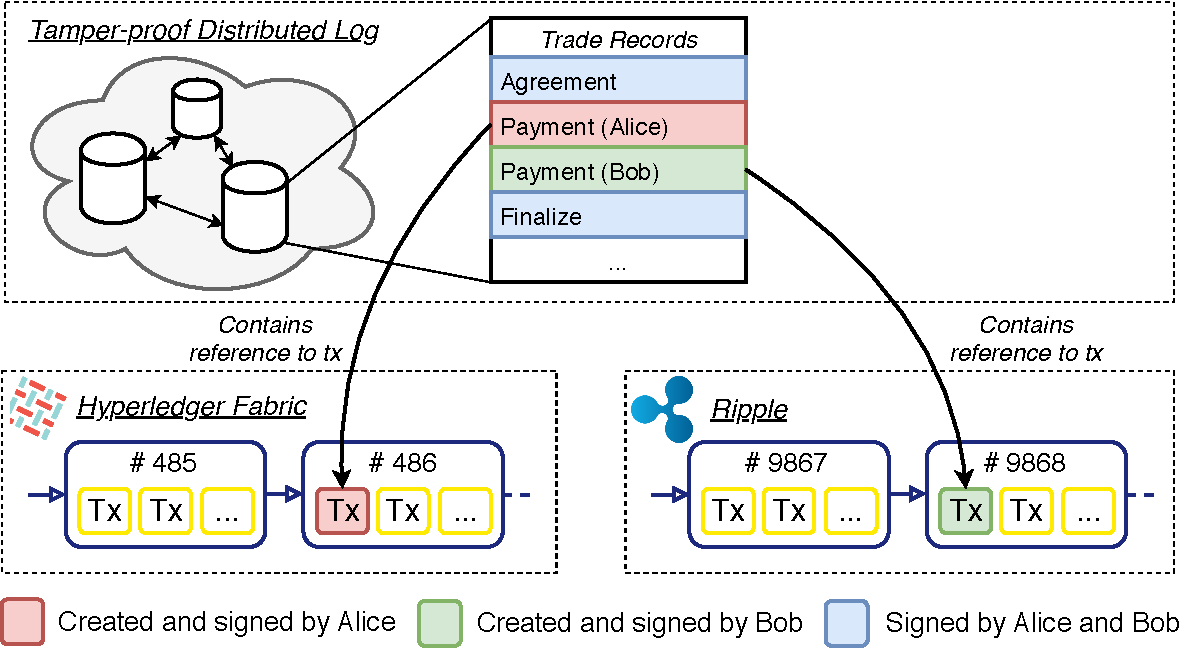
\includegraphics[width=.75\linewidth]{xchange/assets/xchange}
	\caption{High-level overview of our \ModelName{} trading mechanism. In this example, Alice sells some FabTokens that are managed by Hyperledger Fabric to Bob, who pays Alice in XRP (Ripple) tokens. Full trade specifications are stored in a distributed log.}
	\label{fig:xchange}
\end{figure}

We address counterparty risk by storing trade records in a tamper-proof distributed log.
The distributed log enables \ModelName{} traders to detect if a party might have committed fraud during an ongoing trade.
We irreversibly store records of every trade, which makes it difficult for a trader to hide the existence of a specific trade or to unilaterally revert the status of an ongoing trade to a prior state.
Each record in the distributed log is digitally signed by its creator.
We envision that the distributed log can also be audited by external authorities to resolve potential disputes that would arise during the trade procedure.
However, we consider the details of such audits beyond the scope of this work.
The technical requirements of the distributed log are later discussed in Section~\ref{sec:system_threat_model}.

We show a part of the distributed log in Figure~\ref{fig:xchange}, highlighting four records that together describe a completed trade between two peers, Alice and Bob.
This trade exchanges some tokens that are managed by a Hyperledger Fabric and a Ripple ledger.
The lower part of Figure~\ref{fig:xchange} shows parts of the Hyperledger Fabric and Ripple ledgers.
A completed trade that has been stored in the distributed log consists of the following three record types:

\begin{enumerate}
	\item An \texttt{Agreement} record contains the specifications of an upcoming trade, e.g., the agreed amount of assets that will be exchanged between the traders.
	It also includes information on which party conducts the first payment during the upcoming trade.
	The \texttt{Agreement} record bears the digital signature of both traders and can be appended to the distributed log by any of the traders.
	We further describe this record type, and the other two record types below, in our protocol description (see Section~\ref{sec:protocol}).
	\item A \texttt{Payment} record contains the details of a specific payment that has been conducted during a trade.
	This record includes the identifier of the newly issued transaction that transfers assets in the involved blockchain network.
	For instance, the \texttt{Payment} record created by Alice in Figure~\ref{fig:xchange} contains a reference to the transaction that she submitted in the Hyperledger Fabric network.
	Likewise, the \texttt{Payment} record created by Bob points to his transaction in the Ripple network.
	By including the identifier of the transaction in this record, the trading counterparty, and other traders, can verify if the payer transferred the assets.
	Others can verify the validity and inclusion of the transaction reference by the \texttt{Payment} record by inspecting the appropriate blockchain.
	\item A \texttt{Finalize} record completes a trade.
	A \texttt{Finalize} record is appended to the distributed log by the party that received the last payment during the completed trade.
\end{enumerate}

In addition to these three record types, \ModelName{} also includes the \texttt{Order}, \texttt{CancelOrder}, and \texttt{CancelTrade} records.
The \texttt{Order} and \texttt{CancelOrder} records are used when creating a new order and when canceling an unfulfilled order, respectively.
These two record types are further discussed in Section~\ref{sec:protocol}.
The \texttt{CancelTrade} record can be appended to the distributed log to unilaterally abort the trade if one of the parties becomes inactive during a trade.
This feature is later discussed in Section~\ref{sec:limit_risk}.

Our solution so far does not address counterparty fraud when exchanging assets.
Even though the distributed log provides traders with an overview of ongoing and finished trades, it does not prevent a trader from conducting counterparty fraud in a trade.
A malicious trader can even commit counterparty fraud with multiple traders, without repercussions.
We now present two risk mitigation strategies that significantly reduce the gains of traders that commit counterparty fraud.

\subsection{Risk Mitigation Strategy I - Incremental Settlement}
\label{sec:incremental_settlement}
The first risk mitigation strategy we introduce is \emph{incremental settlement}, where a trade is incrementally completed by dividing each payment in $ k $ near-equal, smaller payments.
For example, in a trade with $ k = 2 $ between parties $ A $ and $ B $, party $ A $ first transfers half of the agreed amount of assets to $ B $.
$ B $ then transfers half of the agreed assets to $ A $.
Traders conduct payments until all assets are exchanged.
The \texttt{Agreement} record associated with the trade contains the value of $ k $ used during asset exchange.
On the one hand, incremental settlement decreases the economic gains for adversarial parties when committing counterparty fraud since they receive partial, intermediate payments.
On the other hand, it prolongs the trade since more transactions must be included on the blockchains that are managing the traded assets.
In general, a trade completed using incremental settlement requires $ 2k $ \texttt{Payment} records in the distributed log.

\begin{figure}[t]
	\centering
	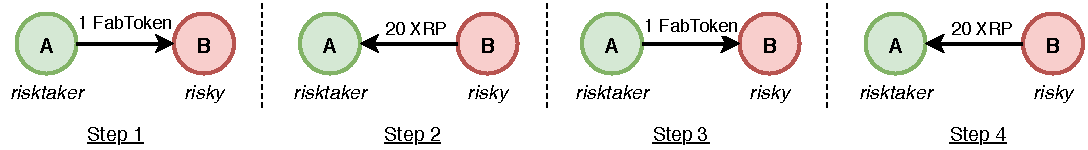
\includegraphics[width=\linewidth]{xchange/assets/trade}
	\caption{An asset exchange with $ k = 2 $ between Alice ($ A $) and Bob ($ B $), trading a total of 2 FabTokens and 40 XRP. During this trade, Alice is the risktaker since she is exposed to counterparty risk. Bob is the risky party since he is able to commit counterparty fraud after step 1 and 3.}
	\label{fig:incremental_trade}
\end{figure}

\subsection{Risk Mitigation Strategy II - Trade Restrictions}
\label{sec:limit_risk}
Our second risk mitigation strategy introduces trade restrictions and ensures that a malicious trader can only commit counterparty fraud once in \ModelName{}.
We achieve this by having traders inspect the distributed log to determine if it is safe to engage in a trade with a particular trading counterparty.
By carefully devising rules that describe when a trader could start a trade with another party, we limit the economic gains of adversarial parties.
In essence, this second risk mitigation strategy forces a trader $ P $ to complete a current, ongoing trade first before others will engage in a trade with $ P $.

To describe the intuition behind our trade restriction rules, we look at a trade between Alice and Bob, where Alice sells 2 FabTokens for 40 XRP, and Bob sells 40 XRP for 2 FabTokens.
Assume that this trade uses incremental settlement with $ k = 2 $, e.g., the total trade consists of four consecutive payments.
Figure~\ref{fig:incremental_trade} visualizes the four payments between Alice and Bob during this trade.
Alice conducts the first payment in this trade.
Notice that after each payment of Bob, the parties are on par with each other.\footnote{We assume here that a trade exchanges an equal amount of value between both traders. In practice, there are usually small profit margins where one party would gain slightly more in value when the trade is complete.} 
Termination of the trade at this state would not cause an economic loss for the parties.
We call this state as \emph{partial complete}.
However, after each payment of Alice, the trade is in a state where Bob has an economic gain and Alice has a loss.
If Bob does not send Alice the promised XRP in return in this state, Bob is said to commit counterparty fraud.
Alice is therefore taking a risk (bounded by $ 40/k $ XRP, i.e.,\ $ 2/k $ FabTokens) after each payment.

%During this trade, Bob could steal assets from Alice and conduct counterparty fraud after steps 1 and 3.
%If Bob stole the FabToken that Alice has sent him and Bob would not send Alice the promised XRP in return, Alice would end up with a net economic loss, whereas Bob has gained economic value.
%However, would Alice compromise Bobs XRP at any point during the trade, she would gain as much advantage as Bob since at that point during the trade both parties sent an equal amount of value to each other.
%In particular, the trade can be considered as a partial complete after step 2 since Alice has now received half of the total XRP, and Bob has received half of the total FabTokens.
%If Alice and Bob agree to abort the exchange asset after step 2, both parties will not suffer an economic loss.

We name the party that is exposed to counterparty risk in a trade a \emph{risktaker}.
%The risktaker is always the party that conducts the first payment in a trade.
The other party is called the \emph{risky} party.
%, since this party could deliberately commit counterparty fraud after having received some assets from the risktaker.
In the example given above, Alice is the risktaker, and Bob is the risky party.

We now introduce three conditions under which a party engages in a trade with another party, based on the records in the distributed log.
As we show later, these conditions prevent a party from being risky in multiple trades at the same time.
%, which would result in the ability of an adversary to commit fraud with potentially many parties.
A party $ C $ will only engage in a trade $ T_2 $ with party $ A $ if at least one of the following three conditions is true:
\begin{enumerate}
	\item $ A $ is currently not involved in a trade, \emph{or}
	\item $ A $ is involved in a trade $ T_1 $ with $ B $ \emph{and} $ A $ is a risktaker in $ T_1 $ \emph{and} it is currently the responsibility of $ B $ to conduct the next payment in $ T_1 $, \emph{or}
	\item $ A $ is involved in a trade $ T_1 $ with $ B $ \emph{and} $ A $ is risky in $ T_1 $ \emph{and} $ A $ is willing to become the risktaker in $ T_2 $.
\end{enumerate}

We visualize these conditions in Figure~\ref{fig:trade_rules}. 
In a nutshell, these conditions prevent the risky party to commit counterparty fraud on more than one parties, and enables the risktaker to involve in other transactions at its own risk.
Specifically, Condition (1) makes it is safe to engage in asset exchange with a trader that is currently not involved in another trade.
This condition can easily be verified by inspection of the distributed log: a party is currently involved in a trade $ T $ when the log contains an \texttt{Agreement} record for $ T $ but no \texttt{Finalize} record (yet).
If all \ModelName{} participants adhere to this rule, a malicious trader cannot commit counterparty fraud more than once.
In particular, as long as one of the parties has a responsibility to conduct a payment to the counterparty during a trade, the party waiting for a payment will refuse to sign a \texttt{Finalize} record for that trade.

With only Condition (1), both parties of an ongoing transaction would be locked out from trading with others until the transaction is finalized.
Conditions (2) and (3) address this case and enables the risktaker to involve in other transactions, at its own risk.
%Conditions (2) and (3) address the case where one of the trading parties becomes inactive.
%For example, during the trade visualized in Figure~\ref{fig:incremental_trade}, Alice can decide not to send the FabToken to Bob before step 1 if she would have second thoughts about the agreed trade.
%Likewise, Bob can decide not to pay Alice the 20 XRP before step 2.
%Under condition (1), both parties are now locked out from trading with others, since other traders detect the incompletion of $ T $.
%This is an unfair situation since the misbehavior of one party during a trade also negatively affects the other party.
%Even though both parties can become inactive during a trade, there are differences when the risktaker or the risky party becomes inactive.
%If the risky party would become inactive, this situation is considered as counterparty \emph{fraud}, since the inactive party now ends up with a positive economic gain.
%When Bob would become inactive after step 1 or step 3 during the trade visualized in Figure~\ref{fig:incremental_trade}, he would end up with 1 FabToken, without having conducted a corresponding payment back to Alice.
%If the risktaker would become inactive at a specific point during a trade, an equal amount of value has been exchanged between the involved parties.
%When Alice becomes inactive before step 1 or step 3, the trade can be considered as partially complete, and no party would be at a loss.
Condition (2) defines the circumstances under which a trader engages in a new trade with another trader that is already a risktaker in an ongoing trade.
If party $ A $ would be an adversary, it cannot commit fraud in its ongoing trade $ T_1 $, and therefore, $ A $ cannot commit counterparty fraud in both $ T_1 $ and $ T_2 $, even if $ A $ acts as the risky party in $ T_2 $.
To discourage $ A $ from becoming inactive in $ T_1 $, we require that $ T_2 $ is in a stage where it is the responsibility of the risky party to conduct the next payment.
Therefore, if $ A $ would become inactive during $ T_1 $ and end up with the responsibility to conduct the next payment, it has to progress $ T_1 $ before $ T_2 $ takes place.
This condition can be verified by inspecting the latest record associated with $ T_1 $ in the distributed log.

Condition (3) defines the circumstances under which a trader $ C $ engages in a new trade with $ A $, while $ A $ is a risky party in an ongoing trade.
Specifically, $ C $ should only trade with $ A $ if in the upcoming trade $ T_2 $, $ C $ becomes the risky party.
This prevents $ A $ from becoming risky in both $ T_1 $ and $ T_2 $.
We remark that all three presented conditions are verified by both parties that intend to trade.
If $ C $ would already be a risky party in a trade, $ A $ detects this and refuse to trade with $ C $.
As a consequence of condition (3), two parties that are both risky in different trades never agree to trade with each other.

A shortcoming of condition (3) is that the trade $ T_1 $ between $ A $ and $ B $ may never complete due to $ A $ being offline.
Therefore, the ability of $ B $ to trade with others is forever restricted by its role as a risky party in $ T_1 $.
To address this situation, we allow a risky party to explicitly cancel an ongoing trade by including a \texttt{CancelTrade} record in the distributed log.
This record can only be included by the risky party, and is only acknowledged by other traders if (1) the risktaker is currently responsible for transferring assets to the risky party during the trade, and (2) at least some time $ \Delta_T $ has elapsed since the last activity in trade $ T $.
The value of $ \Delta_T $ should be well above the confirmation times of transactions submitted to the involved blockchains, to avoid the situation where one might consider a trade as stale while a transaction is still being finalized in the involved blockchain.
When a trade is canceled, no further assets should be exchanged, and the trade is considered as partially complete.
After the risky partner canceled participation in a trade, it loses its risky status and can participate in other trades.

\begin{figure*}[t]
	\centering
	\begin{subfigure}[t]{.33\textwidth}
		\centering
		\captionsetup{width=.9\linewidth}
		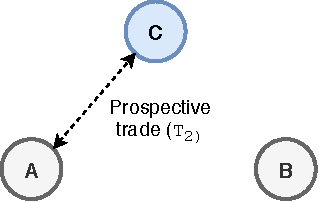
\includegraphics[width=.9\linewidth]{xchange/assets/trade_1}
		\caption{Trader $ C $ will always trade with another party that is not involved in a trade.}
		\label{fig:trade_1}
	\end{subfigure}%
	\begin{subfigure}[t]{.33\textwidth}
		\centering
		\captionsetup{width=.9\linewidth}
		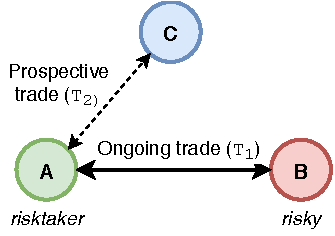
\includegraphics[width=.9\linewidth]{xchange/assets/trade_2}
		\caption{Trader $ C $ will only start $ T_2 $ with a risktaker $ A $ if it is $ B $'s responsibility to conduct the next payment during $ T_1 $.}
		\label{fig:trade_2}
	\end{subfigure}%
	\begin{subfigure}[t]{.33\textwidth}
		\centering
		\captionsetup{width=.9\linewidth}
		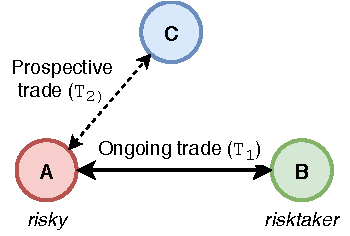
\includegraphics[width=.9\linewidth]{xchange/assets/trade_3}
		\caption{Trader $ C $ will only start $ T_2 $ with risky party $ A $ if $ A $ is willing to act as risktaker in $ T_2 $.}
		\label{fig:trade_3}
	\end{subfigure}
	\caption{Visualization of the trade restriction rules that prevent an adversary from becoming risky in two simultaneous trades. This limits the economic gains of adversaries.}
	\label{fig:trade_rules}
\end{figure*}

%We summarize and visualize the three presented conditions in Figure~\ref{fig:trade_rules}.
As we will prove in Section~\ref{sec:analysis}, Conditions (1)-(3) are sufficient to prevent an adversarial party from being risky in simultaneous trades with honest traders, which effectively limits the economic gains of adversarial parties.
We remark, however, that a trader can always ignore these conditions and engage in other trades \emph{at its own risk}.
Doing so, however, does not provide restrictions on the economic gains of adversarial parties but it enables participants to engage in trade with traders that it already trusts.
Trades that parties started at their own risk do not restrict the involved traders from engaging in new trades with other parties at the same time.
These trades also contain a flag in the associated \texttt{Agreement} record.

\subsection{Accurate Trade Inspections}
Our solution described so far requires other traders to verify whether a specific trader is currently involved in a trade and, if so, if it is their responsibility to conduct the next payment during this trade.
However, a trader can create a \texttt{Payment} record that includes the identifier of a non-existent or invalid transaction in the involved blockchain.
Therefore, traders cannot accurately decide the current state of a trade merely based on the records in the distributed log since a trader can make false claims.
In some situations, traders must perform an additional verification step by inspecting the validity of a transaction on connected blockchains.
Suppose an ongoing trade $ T $ between $ A $ and $ B $, where $ A $ sells some assets $ a $ and $ B $ sells some assets $ b $.
These assets are managed by blockchains $ \mathcal{B}_a $ and $ \mathcal{B}_b $, respectively.
Now, to verify whether a trader $ C $ can open a trade with $ A $, a trader has to inspect the validity of a particular transaction in $ \mathcal{B}_a $ or $ \mathcal{B}_b $ in the following two situations:

\begin{enumerate}
	\item The latest record associated with $ T $ in the distributed log is a \texttt{Payment} record.
	To verify that the creator of this record conducted the payment, $ C $ has to verify the existence and validity of the transaction to which the \texttt{Payment} record points.
	\item The latest record associated with $ T $ in the distributed log is a \texttt{CancelTrade} record.
	$ C $ has to verify that the creation of this record adheres to the trade cancellation rules that we discussed in Section~\ref{sec:limit_risk}.
	To determine this, $ C $ potentially has to check the validity of the latest \texttt{Payment} record associated with $ T $.
\end{enumerate}

It might be that $ C $ does not have the appropriate credentials to read transactions in $ \mathcal{B}_a $ or $ \mathcal{B}_b $, and therefore is unable to determine if a \texttt{Payment} or \texttt{CancelTrade} record by party $ A $ is legitimate.
If $ C $ is unable to determine the legitimacy of the trade record, $ C $ refuses to trade with $ A $, since the claims of $ A $ cannot be accurately verified.
This issue could be resolved by having a special peer, or \emph{gateway}, for each connected blockchain that can be queried by traders when one wants to verify the existence and validity of a transaction on a particular blockchain.
We consider the question on how to build such a gateway beyond the scope of this work.

% Key insight: only one party can effectively commit fraud, depending on who "goes first"
% This party is called risky. For each trade, there is a risky and a non-risky party.
% A counterparty can explicitly cancel a trade if it falls victim to griefing.
% A risky party can remove its risky status by:
%		1) completing the trade
%		2) completing its obligations to the counterparty, putting the trade in a "neutral" state, and posting a "cancel" transaction.

% Someone will always trade with someone else that is not involved in a trade.
% When will someone trade with a non-risky party A?
%		When there is recent progress by A (an outgoing payment)
% When will someone trade with a risky party B?
%		If it is the responsibility of A to act in a trade (requires deep trade inspection)

%\begin{enumerate}
%\item \textbf{Limit the number of ongoing trades}. In \ModelName{}, a trader will only engage in a trade with some counterparty $ c $ if $ c $ is either not currently involved in a trade with another party, or the ongoing trade involving $ c $ is \emph{stale}, and trade staleness is not due to $ c $.
%A stale trade in the context of \ModelName{} is a trade that has not progressed for a pre-defined amount of time, and where it is likely that one of the parties is either offline or has compromised assets from the trading counterparty.
%Before one can engage in another trade, they must finish its ongoing trade first.
%This restriction acts as a punishment for adversarial parties since it prevents further economic activity until their current trade has been completed.
%Since we assume well-established identities (see Section~\ref{sec:system_threat_model}), an adversarial trader cannot easily re-enter the network under a different identity.
%If $ c $ nonetheless is able to convince multiple traders to engage in a trade, integrity constraints enforced by the blockchain will ensure that $ c $ can only start a single trade.
%We remark that a trader can still start a trade \textit{at its own risk} with a party currently involved in another trade.
%This enables high-reputed traders to engage in multiple trades at once.
%\end{enumerate}

%The implementation of the \ModelName{} trading mechanism compromises of a five-phase trading protocol and a system architecture.
%The formal specifications of the trading protocol are given in the next section whereas the system architecture of \ModelName{} is elaborated in Section~\ref{sec:architecture}.

\section{System Assumptions and Threat Model}
\label{sec:system_threat_model}
We first discuss the \ModelName{} system model.
This includes our assumptions on the blockchains that are managing the assets being exchanged, the requirements of the distributed log used by \ModelName{}, and the specifications of the underlying \ModelName{} network.
We then present the threat model of \ModelName{}, and state the goals and capabilities of adversarial parties.

\subsection{Blockchain, Distributed Log, and Network Specifications}
\label{sec:blockchain_network_specs}
The \ModelName{} mechanism coordinates asset exchange between permissioned blockchains.
W.l.o.g., we denote the blockchains that are managing the assets being exchanged by $ \mathcal{B}_a $ and $ \mathcal{B}_b $ respectively.
\ModelName{} only requires that $ \mathcal{B}_a $ and $ \mathcal{B}_b $ can represent assets and transfer assets to another owner.
The consensus mechanisms deployed by $ \mathcal{B}_a $ and $ \mathcal{B}_b $ might be fundamentally different.
We assume that for each involved blockchain, the fraction of adversarial parties is bound by the threshold necessary to ensure safety and liveness properties.
In PBFT-based consensus algorithms, this threshold is usually $ \frac{1}{3} $ of all nodes involved in the consensus algorithm~\cite{castro1999practical}.

\ModelName{} stores trade records in a distributed log, denoted by $ \mathcal{L} $.
We require that the entries stored by $ \mathcal{L} $ are immutable and append-only.
If entries in $ \mathcal{L} $ would be mutable or can be removed, a trader could trick a counterparty into starting a trade, commit counterparty fraud, and remove all traces of the trade.
Similar to how participation in $ \mathcal{B}_a $ and $ \mathcal{B}_b $ is explicitly approved, participation in $ \mathcal{L} $ should be managed by an authority.
We envision that a trader joining \ModelName{} re-uses the well-defined identity under which it participates in one of the permissioned blockchains.
We remark that $ \mathcal{L} $ can, for example, be realized through a blockchain with support for smart contracts.

Users in \ModelName{} participate in a peer-to-peer network, which is used to send point-to-point messages to other users.
This network is particularly used during trade negotiation, as we further specify in Section~\ref{sec:protocol}.
We assume that peers in the \ModelName{} network know the network addresses of other peers.

\subsection{Peer Model}
We now elaborate on the assumptions of peers participating in \ModelName{}.

Each peer in the \ModelName{} network owns a cryptographical key pair consisting of a public and a private key. 
The public key of a specific peer is known to others and uniquely identifies it in the network. 
Their private key is used to digitally sign data such as records appended to $ \mathcal{L} $, or outbound messages in the peer-to-peer network.

As we discussed in Section~\ref{sec:blockchain_network_specs}, the digital identity of each peer in the \ModelName{} network uniquely identifies a real-world user.
Identity validation should be performed by a Registration Authority (RA), which is external to our system.
The RA could be the same authority that approved participation in $ \mathcal{B}_a $ or $ \mathcal{B}_b $.
We assume that the RA does not collude with traders in \ModelName{}.
In \ModelName{}, well-established digital identities are necessary to prevent misbehaviors such as a Sybil Attack and a distributed denial-of-service attack~\cite{douceur2002sybil,Specht2004DistributedDO}.
We also use verified identities for accountability purposes, where misbehavior in a trade can be traced back to a real-world persona.

Whereas existing work primarily focuses on \emph{how} assets are exchanged, the \ModelName{} mechanism also includes primitives for traders to specify trade interest through orders, and to find trading partners that can fulfill these orders.
We distinguish between \emph{makers} and \emph{takers}.
A maker is a peer that creates a specific order, whereas a taker is a peer that fulfills an order.
Makers introduce trading opportunities and liquidity to the \ModelName{} network.
A peer in \ModelName{} can act as both maker and taker, for distinct orders.
The maker-taker order model is also adopted by related protocols that enable the exchange of tokens on the Ethereum blockchain, namely 0x and AirSwap~\cite{warren20170x,airswap}.

\subsection{Threat Model}
Adversarial parties in \ModelName{} aim to \emph{maximize their economic gains} by committing counterparty fraud in ongoing trades.
Adversarial parties could attempt to append invalid records to $ \mathcal{L} $, intentionally ignore incoming messages in the peer-to-peer network, or refuse to respond to messages during trade negotiation.
They also could strategically ignore the risk mitigation strategies described in Section~\ref{sec:limit_risk}.
We assume that adversaries cannot compromise the integrity of the distributed log $ \mathcal{L} $ used by \ModelName{} and cannot undermine the security of the blockchains that are hosting the assets being traded, $ \mathcal{B}_a $ or $ \mathcal{B}_b $.
We also assume that the cryptographic primitives used by all involved blockchains are secure (e.g., digital signatures cannot be forged) and that the computational capabilities of adversaries are bounded.

\section{The \ModelName{} Trading Protocol} \label{sec:protocol}
We now present the \ModelName{} trading protocol for asset exchange between permissioned blockchains and specify all operations conducted by peers that are participating in a trade.
We assume the system and threat model described in the prior section.
The protocol consists of four phases.
In the first phase, makers specify their trade interest by appending new orders to the distributed log $ \mathcal{L} $.
During the second phase, takers negotiate with makers about orders they would like to fulfill and append an \texttt{Agreement} record to the distributed log when they reach an agreement.
During the third phase, the maker and taker execute the trade by exchange assets through payments.
The trade is finalized in the fourth phase with a \texttt{Finalize} record.

\begin{figure}[h]
	\centering
	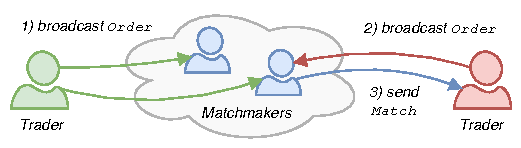
\includegraphics[width=0.6\linewidth]{xchange/assets/xchange_protocol_1}
	\caption{Phase I of the \ModelName{} trading protocol: makers (depicted in green) indicate trade interests by appending an \texttt{Order} record to the distributed log.}
	\label{fig:matching_protocol_1}
\end{figure}

\subsection*{Phase I: Order Creation and Cancellation}
\label{sec:phase_matching}

During the first phase of the \ModelName{} protocol, makers create new orders and append these orders to $ \mathcal{L} $, see Figure~\ref{fig:matching_protocol_1}.
When a trader intends to buy or sell some assets, it constructs a new order which we denote by $ O $.
$ O $ contains details on the quantity and the type of assets that the maker desires to buy and sell.
The order creator provides this information as a two-tuple of asset quantities, also called an \emph{asset pair}.
The first asset quantity in the asset pair indicates the assets that the order creator wants, and the second asset quantity indicates what the order creator offers in return.
An asset quantity is described by the combination of an integer value and a string that indicates the asset type.
For example, if a trader intends to sell 2 FabTokens for 40 XRP tokens, it creates an order with asset pair ($ 2 $ FabToken, $ 40 $ XRP).

$ O $ includes an integer value, $ k $, that specifies the order creator's preference regarding the number of partitions each payment is divided in.
As discussed in Section~\ref{sec:incremental_settlement}, one way how \ModelName{} reduces value at stake is by using incremental settlement.
The inclusion of $ k $ in $ O $ indicates the risk that the maker is willing to take in an upcoming trade that fulfills $ O $ if the order creator would become the risktaker.
Furthermore, $ O $ includes the address of the wallet in which the order creator wishes to receive assets from a prospective trader during an upcoming trade.
By including this information, a taker knows to which address it should transfer its assets.
This information is also used by other traders to verify if the maker has received assets from a taker.

We observe that a maker may create a \enquote{fake} order that specifies interest to sell assets that the maker does not possess.
Essentially, this order provides non-existent liquidity to the \ModelName{} network, since a trade fulfilling the fake order will never complete.
We address the creation of orders that are not backed by real assets by requiring a \emph{proof-of-ownership} in each new order.
A proof-of-ownership proves that a specific peer holds ownership over assets managed by some blockchain $ \mathcal{B}_a $.
This proof is represented as a combination of a public key and a digital signature over the order content in serialized form.
To generate this signature, the order creator should use the cryptographic key pair associated with the account on $ \mathcal{B}_a $ that holds the assets that the order creator intends to sell.
Takers verify the proof-of-ownership to check that the order creator could complete a prospective trade, and owns the assets it intends to sell.

After adding all required fields to $ O $, the order creator serializes the order and embeds it in an \texttt{Order} record.
The order creator then appends the \texttt{Order} record to $ \mathcal{L} $.
The order identifier can be determined by taking the hash of the record content, which we denote by $ H(O) $.

A maker can cancel any of their non-expired orders that are not being fulfilled by an ongoing trade.
This is achieved by the maker appending a \texttt{CancelOrder} record containing $ H(O) $ to $ \mathcal{L} $.

\begin{figure}[h]
	\centering
	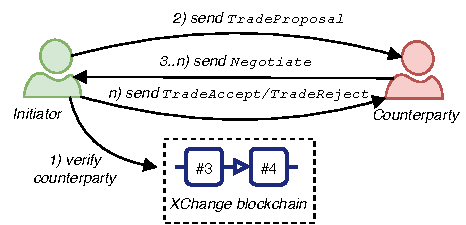
\includegraphics[width=0.6\linewidth]{xchange/assets/xchange_protocol_2}
	\caption{Phase II of the \ModelName{} protocol: a maker and taker negotiate a trade agreement. Upon a successful negotiation outcome, a dual-signed \texttt{Agreement} record will be appended to the distributed log.}
	\label{fig:matching_protocol_2}
\end{figure}

\subsection*{Phase II: Trade Negotiation}
\label{sec:phase_clearing}

During the second phase of the \ModelName{} trading protocol, a maker and taker negotiate a trade, see Figure \ref{fig:matching_protocol_2}.
If the negotiating maker and taker agree to trade, one of the parties appends this agreement to $ \mathcal{L} $.
We now describe this negotiation process.

This phase starts when a taker discovers an order $ O $, included on $ \mathcal{L} $, that it wishes to fulfill.
Assume that this order has been created by a maker $ M $.
Before sending a trade proposal to $ M $, the taker performs three checks that determine if the taker should trade with $ M $.
First, the taker checks if it is willing to trade with $ M $ as a person.
For instance, $ M $ could have attempted to commit counterparty fraud in the past, which could be a reason for the taker to refrain from trading with $ M $.
Second, the taker determines the validity of the proof-of-ownership included in $ O $ to ensure that $ M $ has sufficient assets to complete an upcoming trade.
Third, the taker determines if it is safe to trade with $ M $, according to the second risk mitigation strategy described in Section~\ref{sec:limit_risk}.
The taker can check whether $ M $ is already involved in a trade by inspecting the latest records on $ \mathcal{L} $ involving $ M $.
If $ M $ is already involved in a trade $ T $, the information on $ \mathcal{L} $ also reveals if $ M $ in $ T $ is a risky party or a risktaker.

When all three checks pass, the taker creates and sends a \texttt{Proposal} message to $ M $.
A \texttt{Proposal} message contains a proposal for $ M $ to fulfill order $ O $.
A taker includes five pieces of information in a \texttt{Proposal} message.
First, it includes the identifier of $ O $, so the maker knows which order the taker wants to fulfill (a trader could have created multiple orders).
Second, the taker includes a proof-of-ownership for the assets it intends to transfer to the maker.
Third, the taker includes its destination wallet address to which $ M $ should send its assets during the trade.
Forth, the taker includes an integer value, $ k $, that indicates how much risk the taker is willing to take if it would become the risktaking party.
Finally, the taker includes a boolean value in the proposal indicating if the taker becomes a risktaker in the upcoming trade.
At a high level, a \texttt{Propose} message represents a new order that indicates the taker's trade preferences.

When $ M $ receives a \texttt{Proposal} message from taker $ T $, it also verifies whether it wants to trade with $ T $.
Specifically, $ M $ performs the same three checks as the taker did.
Furthermore, $ M $ verifies if it agrees with the role classification proposed by the taker.
If validation fails, the maker immediately sends a \texttt{Reject} message back to the taker, containing the identifier of the rejected order and, optionally, why $ M $ has rejected the proposal.
If $ M $ agrees with the proposal and also wishes to trade with $ T $, $ M $ constructs a \texttt{Agreement} record, which includes the identifier of the order being fulfilled and the proposal created by the taker (including the taker's signature).
This \texttt{Agreement} record is signed by $ M $, sent back to $ T $, and appended to $ \mathcal{L} $.
Inclusion of the \texttt{Agreement} record on $ \mathcal{L} $ binds the maker and the taker to the trade agreements.
Since the risktaker is exposed to counterparty risk in the upcoming trade, the preferred value of $ k $ by the risktaker is used during the upcoming asset exchange.
If the maker is the risktaker, the value of $ k $ as specified in the \texttt{Order} record describing $ O $ is leading.
Otherwise, if the taker becomes the risktaker, the value of $ k $ specified by the taker in its proposal is leading.

\begin{figure}[h]
	\centering
	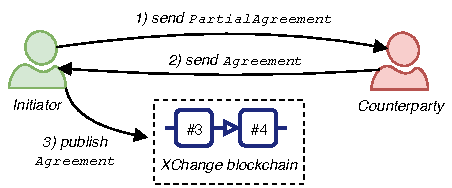
\includegraphics[width=0.68\linewidth]{xchange/assets/xchange_protocol_3}
	\caption{Phase III of the \ModelName{} protocol: a maker and taker trade by exchanging assets. In this trade, the taker is the risktaker (initiating the first payment) and the maker is the risky party.}
	\label{fig:matching_protocol_3}
\end{figure}

\subsection*{Phase III: Trade Settlement}
\label{sec:phase_settlement}
During the third phase of the \ModelName{} trading protocol, assets are exchanged between the maker and taker, and the trade is settled.
Figure~\ref{fig:matching_protocol_3} visualizes a trade between a maker and taker, with $ k = 1 $, where the maker sells FabTokens, a token managed by Hyperledger Fabric, and gets XRP (Ripple) tokens in return from the taker.
This trade, fulfilling order $ O $, consists of two payments, one from the maker to the taker, and one from the taker to the maker.

Asset exchange starts by the risktaker (the taker in this specific example) issuing a transaction to the Ripple network managing the XRP tokens.
This Ripple transaction transfers XRP tokens from the wallet associated with the proof-of-ownership in the \texttt{Proposal} message to the wallet address that was specified by the maker in the \texttt{Order} record associated with $ O $.
After the taker has issued this transaction in the Ripple network, it appends a \texttt{Payment} record to $ \mathcal{L} $, which contains the identifier of the order being fulfilled, and the identifier of Ripple transaction.
The \texttt{Payment} record allows the maker (and other traders) to verify that the taker has transferred the correct amount of assets to the maker.

After the maker has verified that it received the agreed amount of XRP tokens, it conducts the next payment by issuing a transaction to the Hyperledger Fabric network.
This transaction transfers FabTokens from the wallet associated with the proof-of-ownership in the \texttt{Order} record to the wallet that was specified by the taker in the \texttt{Proposal} message.
The maker then appends a \texttt{Payment} to $ \mathcal{L} $, which includes the identifier of the transaction in the Hyperledger Fabric network.
This payment process repeats until all assets have been exchanged between the maker and the taker.

There is a risk that a trade does not progress when one of the traders becomes inactive.
As pointed out in Section~\ref{sec:limit_risk}, a stale trade is only a minor concern for the risktaker since this party can still engage in other trades after $ \Delta_T $ time has elapsed.
A risky party can explicitly cancel an ongoing trade to dismiss its responsibility as a risky party by appending a \texttt{CancelTrade} record to $ \mathcal{L} $.
This record only contains the identifier of the order currently being fulfilled.
Other traders should verify that the \texttt{CancelTrade} adheres to the rules as outlined in Section~\ref{sec:limit_risk}, to prevent the risky party from illegally canceling a trade after having committed counterparty fraud.

\begin{figure}[h]
	\centering
	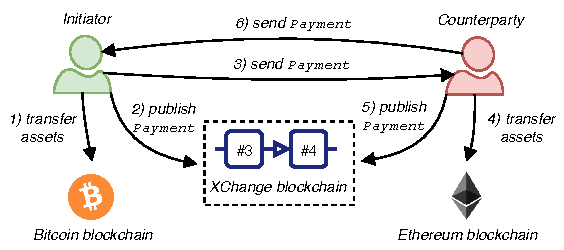
\includegraphics[width=0.6\linewidth]{xchange/assets/xchange_protocol_4}
	\caption{Phase IV of the \ModelName{} protocol: the taker finalizes the trade.}
	\label{fig:matching_protocol_4}
\end{figure}

\subsection*{Phase VI: Trade Finalization}
\label{sec:phase_finalization}
When all assets have been exchanged, the party receiving the final payment during a trade creates a \texttt{Finalize} record and appends it to $ \mathcal{L} $, see Figure~\ref{fig:matching_protocol_4}.
Since the risky party conducts the final payment during a trade, finalization is always performed by the risktaker.
Inclusion of a \texttt{Finalize} record on $ \mathcal{L} $ completes a trade, say $ T_1 $, between the maker and taker, and both parties can now start new trades with others.
%One might argue that an explicit finalization is redundant since a trader can determine if $ T_1 $ is complete by counting the number of issued \texttt{Payment} records during the trade.
%However, the risky party might include a \texttt{Payment} transaction without actually having transferred the assets, which can falsely trick other users into thinking that the trade has been successful.
%A \texttt{Finalize} record indicates that the trade has explicitly been finished by both parties and that both parties acknowledge that the trade is complete.
%Note that if the risktaker waits too long with submitting a \texttt{Finalize} record after a trade has been complete, it is considered as griefing after some time has elapsed.

\section{Security Analysis}
\label{sec:analysis}
We now analyze the security of the \ModelName{} mechanism.
First, we prove that the economic gains of adversarial parties committing counterparty fraud are limited.
We then discuss the scenario where multiple adversaries collude to gain an advantage as a group.

\subsection{Counterparty Fraud Limitations}
We further analyze our second risk mitigation strategy presented in Section~\ref{sec:limit_risk}.
This risk mitigation strategy defines conditions under which an honest party should could a new trade with another party that already might be involved in a trade.
Our analysis focuses on the following statement: \emph{an adversary cannot become a risky party in simultaneous trades with honest parties.}
If this statement is true, an adversary would first have to finish an ongoing trade in which it was risky before the adversary can start a new trade in which it is also risky.
As a result, an adversary can only commit counterparty fraud once in simultaneous trades with honest traders.
This property, therefore, limits the economic gains of adversaries.

We now analyze the correctness of the statement above.
Assume a trade $ T_1 $ with $ k = 2 $ between an honest trader $ A $ and an adversarial trader $ B $.
Recall that honest traders follow the \ModelName{} protocol and therefore verify the conditions stated in Section~\ref{sec:limit_risk} before starting a new trade.
Assume that in $ T_1 $, $ A $ is the risktaker, and $ B $ is the risky party.
We explore possibilities for trader $ B $ to commit counterparty fraud with multiple, honest traders.
Assume that $ A $ has just conducted the first payment to $ B $ and appended a \texttt{Payment} record to the distributed log.
At this point, $ B $ can commit counterparty fraud in $ T_1 $ in two ways.
First, it can choose to become inactive in $ T_1 $ and not conduct a payment back to $ A $.
Second, $ B $ could append a \texttt{Payment} record to $ \mathcal{L} $ that points to a non-existent or invalid transaction, attempting to trick $ A $ (and other traders) that $ B $ has conducted a payment back to $ A $.

Given that $ B $ commits counterparty fraud, we consider now what happens if $ B $ attempts to open a new trade $ T_2 $ with another honest trader $ C $.
Specifically, $ B $ intends to become a risky party during $ T_2 $, so it can commit counterparty fraud again.
Since $ C $ is honest, $ C $ will verify whether it could trade with $ B $ according to the \ModelName{} risk mitigation strategies.
When $ C $ inspects the status of $ B $ based on the included records on $ \mathcal{L} $, it will discover the ongoing trade $ T_1 $ between $ A $ and $ B $, and learn that $ B $ is the risky party in $ T_1 $.
Condition III described in Section~\ref{sec:limit_risk} states that $ C $ will only agree to engage in $ T_2 $ with $ B $ if $ B $ becomes the risktaker and $ C $ becomes the risky party in $ T_2 $.
In this situation, $ B $ would be unable to commit counterparty fraud in $ T_2 $.
Therefore, $ B $ is unable to take on the role of a risky party in another trade and thus is unable to commit counterparty fraud in both $ T_1 $ and $ T_2 $.

We now analyze the situation where $ B $ cancels its ongoing trade $ T_1 $ by appending a \texttt{CancelTrade} record to $ \mathcal{L} $, after having committed counterparty fraud.
When $ C $ considers entering in trade $ T_2 $ with $ B $, it will discover the \texttt{CancelTrade} record in $ \mathcal{L} $ and checks that the trade cancellation by $ B $ is legitimate and adheres to the rules.
Recall that the cancellation of trade $ T_1 $ by $ B $ is legitimate if it is currently the responsibility of the risktaker to conduct the next payment.
The trade cancellation of $ T_1 $ is not valid since $ B $ has committed counterparty fraud.
If the trade cancellation were legit, $ B $ would not have committed counterparty fraud in $ T_1 $ since it then transferred assets back to $ A $.
Now, when $ C $ verifies the status of $ B $, it detects that $ B $ has canceled its last trade and detect that the trade cancellation is not legit.
Therefore, $ C $ will not engage in trade $ T_2 $ with $ B $.

Our analysis shows that $ B $ is not able to engage as a risky party in simultaneous trades with honest parties.
This limits the economic gains of adversaries.
Adversaries that have committed fraud in an ongoing trade first have to finish that trade, nullifying the gains of the fraud, before others agree to trade with the adversarial party.

\subsection{Collusion Resistance}
In a collusion attack, a group of traders follows a common strategy to subvert the network or gain advantages as a collective.
The \ModelName{} mechanism is highly resistant against collusion attacks since adversarial parties are not able to gain more economic gains when working together, given that $ \mathcal{L} $ provides secure storage of included trade records.
We argue that the resistance against collusion can be addressed to the absence of group-based coordination in \ModelName{}.
Tasks that would involve coordination among a group are usually vulnerable to attacks where a majority of the group colludes to gain advantages over non-colluding users.
In \ModelName{}, trade proceeds through the direct interaction between the involved traders and therefore, cannot be influenced by groups of colluding adversaries.

\section{Distributed Logging of Trade Records}
\label{sec:blockchain_accounting}
The \ModelName{} trading protocol described in Section~\ref{sec:protocol} requires a distributed log to securely and irreversibly store \texttt{Order}, \texttt{CancelOrder}, \texttt{Agreement}, \texttt{Payment}, \texttt{Finalize} and \texttt{CancelTrade} records.
We choose to build \ModelName{} upon TrustChain~\cite{otte2017trustchain} which is a shared data structure with a sharp focus on tamper-resilience and trustworthy record storage.
In this section, we motivate our choice for TrustChain and outline how TrustChain is used to store \ModelName{} records.

\subsection{TrustChain: A Scalable Ledger for Accounting} \label{sec:trustchain}
Based on the idea of blockchain ledgers that order transactions in a directed acyclic graph (DAG), Otte et al. designed, implemented, and deployed TrustChain.
TrustChain is a ledger that is optimized for lightweight, tamper-proof accounting of data elements~\cite{otte2017trustchain}.
The key idea is that individuals maintain and grow their \emph{individual ledger} with records.
Other users verify these records according to some pre-defined rules.
This makes TrustChain similar to solutions for tamper-proof, distributed logging, such as PeerReview~\cite{haeberlen2007peerreview}.
TrustChain does not aim to prevent integrity attacks on the data structure, e.g., fork creation, but instead guarantees eventual \emph{detection} of these attacks.
This yields superior scalability compared to other ledgers but allows for the situation where some malicious activity targeted at the ledger might go undetected for some time, for example, the hiding of specific transactions.
In TrustChain, this can be addressed by waiting longer before accepting a record as valid.
Individuals in TrustChain are not required to store all records in the network and might choose to store different parts of the global DAG ledger.
TrustChain does not reach a global consensus over all records but relies on participants to detect inconsistencies in individual ledgers.

\begin{figure*}[t]
	\centering
	\begin{subfigure}[t]{.33\textwidth}
		\centering
		\captionsetup{width=.9\linewidth}
		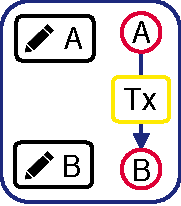
\includegraphics[width=.35\linewidth]{xchange/assets/trustchain_tutorial_1}
		\caption{A block with a record (\emph{R}) between two users ($ A $ and $ B $). Each block contains a single record, two digital signatures and two digital identities.}
		\label{fig:trustchain_tutorial_1}
	\end{subfigure}%
	\begin{subfigure}[t]{.33\textwidth}
		\centering
		\captionsetup{width=.9\linewidth}
		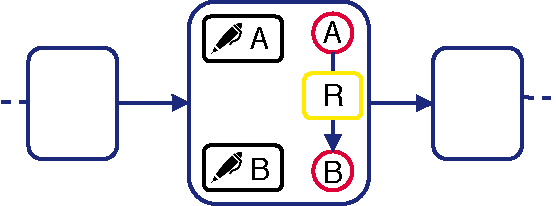
\includegraphics[width=\linewidth]{xchange/assets/trustchain_tutorial_2}
		\caption{An individual ledger. Each block in the chain contains a hash that describes the prior block.}
		\label{fig:trustchain_tutorial_2}
	\end{subfigure}
	\par\bigskip
	\begin{subfigure}[t]{.33\textwidth}
		\centering
		\captionsetup{width=.9\linewidth}
		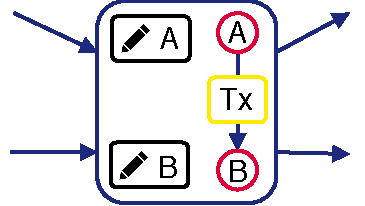
\includegraphics[width=.7\linewidth]{xchange/assets/trustchain_tutorial_3}
		\caption{To increase security, each block also references the previous block in the chain of a record counterparty.}
		\label{fig:trustchain_tutorial_3}
	\end{subfigure}
	\begin{subfigure}[t]{.33\textwidth}
		\centering
		\captionsetup{width=.9\linewidth}
		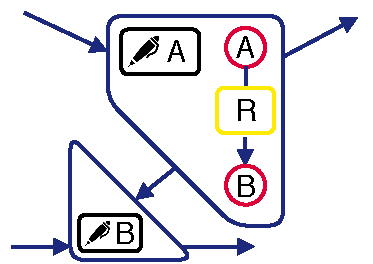
\includegraphics[width=.71\linewidth]{xchange/assets/trustchain_tutorial_4}
		\caption{To improve scalability, we extend the TrustChain structure to support concurrent block creation.}
		\label{fig:trustchain_tutorial_4}
	\end{subfigure}\hspace{0.05\textwidth}%
	\caption{Storing records in TrustChain.}
	\label{fig:trustchain_tutorial}
\end{figure*}

We argue that TrustChain is a suitable ledger to store \ModelName{} records, for the following four reasons.
First, TrustChain allows participants to verify the integrity of other individual ledgers themselves, and determine whether a party is already involved in a trade or not.
There is no requirement to reach a global consensus on the integrity of included records.
Second, TrustChain does not require network-wide replication of all records but enables individuals to selectively share parts of their individual ledger with others.
This feature reduces storage requirements and allows \ModelName{} to also run on devices with storage limitations, as we demonstrate in Section~\ref{sec:exp_trading_low_devices}.
Third, the TrustChain structure is optimized to store bilateral records that are signed by two parties.
This aligns well with the \ModelName{} trading protocol since many operations could benefit from support for bilateral records (for example, trade agreements).
Finally, TrustChain is already being used by various decentralized applications that require accounting features, such as self-sovereign identities~\cite{pouwelse2017laws}.
At the time of writing, the public TrustChain ledger contains over 110 million records, created by 66.377 unique identities.\footnote{See http://explorer.tribler.org}

\subsection{Storing TrustChain Records}
We now outline how a record between two interacting users $ A $ and $ B $ is recorded in TrustChain, see Figure \ref{fig:trustchain_tutorial}.
Each record is stored within a block.
Figure \ref{fig:trustchain_tutorial_1} highlights one block containing a record between $ A $ and $ B $.
Each block contains a single record (\emph{R}).
A record can be a generic description of any interaction between users, for instance, a trade agreement or a payment.
Both interacting parties digitally sign the block with the record by using any secure digital signing algorithm.
These signatures are included in the block and ensure that participation by both parties is irrefutable.
It also confirms that both parties agree with the record itself.
Others can effectively verify the digital signatures included in a block.
After all required signatures have been added to a block, the block is committed to the local databases of the two interacting parties.

The security of stored blocks is improved by linking them together, incrementally ordered by creation time.
In particular, each block is extended with a description (hash) of the previous block.
Each block has a sequence number that indicates its position in the individual ledger.
This results in the structure shown in Figure \ref{fig:trustchain_tutorial_2}.
As a result, each user maintains their individual ledger, which contains all records in which they have participated.
This sets TrustChain apart from the structure of traditional blockchains, where the entire network maintains a single, linear ledger.

Note how the blockchain structure in Figure \ref{fig:trustchain_tutorial_2} allows $ A $ to modify blocks in their individual ledger without being detected by others.
In particular, $ A $ can reorder the blocks in its individual ledger since validity can quickly be restored by recomputing all hashes.
In most blockchain applications, the global consensus mechanism prevents this kind of manipulation.
TrustChain uses a more efficient approach: each block is extended with an additional (hash) pointer that points to the previous block in the individual ledger of the counterparty.
This is visualized in Figure \ref{fig:trustchain_tutorial_3}.
Each block now has exactly two incoming and two outgoing (hash) pointers, except for the last block in an individual ledger, which only has two incoming pointers.
Modifications of the individual ledger by $ A $, like reordering or removing blocks, can now be detected by one or more counterparties.
To prove this fraud, a counterparty reveals both the correct block and the invalid block created by $ A $.

When two parties transact and create a block, their chains essentially become entangled.
When users create more records with others, it leads to the directed acyclic graph (DAG) structure, as shown in Figure \ref{fig:trustchain}.
Figure \ref{fig:trustchain} shows seven blocks, created by seven unique users.
Each block is added once to the individual ledger of all parties involved in the record.
For a more advanced analysis of the technical specifications and security of TrustChain, we refer the reader to the original paper by Otte et al.~\cite{otte2017trustchain}.

\begin{figure}[t]
	\centering
	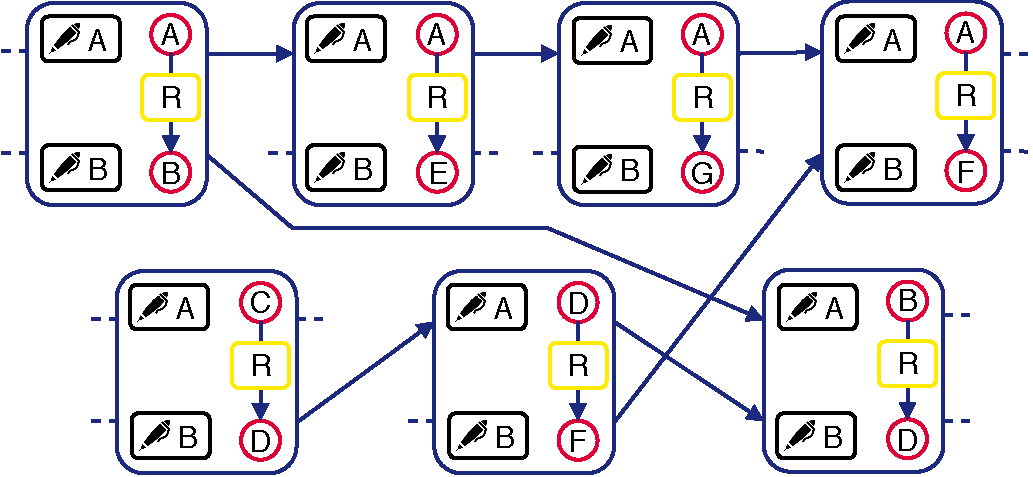
\includegraphics[width=.6\linewidth]{xchange/assets/trustchain}
	\caption{The TrustChain ledger, with seven blocks created by seven participants.}
	\label{fig:trustchain}
\end{figure}

\subsection{Improving TrustChain Scalability}
According to Otte et al., TrustChain is designed to scale~\cite{otte2017trustchain}.
However, we identify that its design limits a user to one pending block creation at once.
The main issue is that the digital signature of a counterparty is required before a new block can be appended to an individual ledger (since the input for the hash of each new block includes all signatures in the previous block).
This enables an attack where a malicious user can purposefully slow down the block creation of others by delaying the signing process of a bilateral transaction it is involved in.
It also limits the growth rate of individual ledgers and reduces the overall scalability of TrustChain.

We contribute to TrustChain and improve its scalability by adding support for \emph{concurrent block creation}.
The idea is to remove the requirement for a digital signature of the counterparty when appending new blocks to an individual ledger.
We believe that this concurrency is necessary since it allows traders to append new records without reliance on other parties.

Our solution is visualized in Figure \ref{fig:trustchain_tutorial_4}.
It shows a record between users $ A $ and $ B $, initiated by $ A $.
We partition a block in two parts, and each block partition is appended to the individual ledger of exactly one party.
Construction of a block between $ A $ and $ B $ now proceeds as follows: first, user $ A $ creates a record by constructing a block partition with the record content and its digital signature.
User $ A $ adds this block partition to its individual ledger immediately (note that it does not include the digital signature of $ B $).
$ A $ now sends the block partition to $ B $.
If $ B $ agrees with the transaction, it signs the block partition created by $ A $, adds it to its individual ledger, and sends his block partition (with their signature) back to $ A $.
User $ A $ stores the block partition created by $ B $ in its local database.
The participation of both parties in this record can now be proven with both block partitions.
This mechanism allows users to be involved in multiple block constructions at once.

\begin{figure}[t]
	\centering
	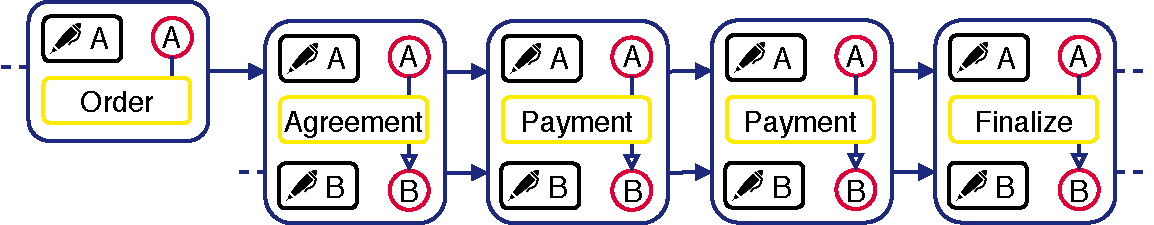
\includegraphics[width=.8\linewidth]{xchange/assets/trustchain_market}
	\caption{A part of the TrustChain ledger, storing an order created by a maker $ A $, and full specifications of a finished trade between $ A $ and $ B $.}
	\label{fig:trustchain_market}
\end{figure}

\subsection{Logging Trade Records on TrustChain}
We now outline how \texttt{Order}, \texttt{CancelOrder}, \texttt{Agreement}, \texttt{Payment}, \texttt{Finalize} and \texttt{CancelTrade} records are stored on TrustChain.
Figure \ref{fig:trustchain_market} shows a part of the TrustChain ledgers of traders $ A $ and $ B $.
It includes a sequence of records that indicate a finished trade between $ A $ and $ B $.
Trade agreements, created during the second phase in the \ModelName{} protocol, are stored within a bilateral \texttt{Agreement} record and digitally signed by both involved traders.
Individual payments are stored within bilateral \texttt{Payment} records.
A \texttt{Payment} record signed by both parties indicates that the payer has conducted the payment and that the payee has observed the payment.
Finally, a trade finalization is stored within a bilateral \texttt{Finalize} record.
Since the overhead of creating new TrustChain records is low, we also store orders as unilateral \texttt{Order} records in individual ledgers.
A unilateral record only contains the digital signature of its creator.
Figure~\ref{fig:trustchain_market} shows a \texttt{Order} record, created by maker $ A $.
Furthermore, \texttt{CancelOrder} and \texttt{CancelTrade} records are also included as unilateral records in one's individual TrustChain ledger.

A particular issue is that the fragmented nature of the TrustChain DAG makes it difficult for takers to discover interesting orders quickly.
Specifically, \texttt{Order} records are by default only stored in the individual ledger of the order creator.
Therefore, we introduce \emph{matchmakers}, peers that continuously collect TrustChain records in the network, and store the information in \texttt{Order} records in a local database.
Matchmakers aggregate orders, and takers can query the database of matchmakers to find interesting orders.
Makers also send their TrustChain blocks with an \texttt{Order} record to known matchmakers after creation.
The role of matchmakers in \ModelName{} is comparable with that of relay nodes in 0x~\cite{warren20170x} and indexers in AirSwap~\cite{airswap}.

\section{Implementation and Evaluation}
\label{sec:evaluation}
In this section, we present the implementation of \ModelName{} and our experimental evaluation.
The evaluation answers the following two questions: (1) what is the overhead of \ModelName{}, in terms of trade duration, when \ModelName{} is deployed on low-resource devices? And (2) How scalable is \ModelName{} in terms of throughput and trade duration when increasing the system load?

\subsection{Implementation Details}
\label{sec:implementation}
We have implemented the \ModelName{} in the Python 3 programming language.
Our implementation spans a total of 4.702 lines of code and uses an event-based programming model, powered by the \texttt{Twisted} library.
The implementation is open source and all software artifacts (source code, tests, and documentation) are published on GitHub.\footnote{https://github.com/tribler/anydex-core}

\textbf{Networking.}
We have built \ModelName{} on top of an existing networking library that is also used by TrustChain.
%Since TrustChain is built upon the IPv8 decentralized networking library, we decided to adopt it for all network communication generated by \ModelName{}.
%Our motivation for this is that TrustChain utilizes the same networking library.
This library provides the functionality to devise decentralized overlay networks and has built-in support for authenticated network communication, custom message definitions, and UDP hole punching.\footnote{https://github.com/tribler/py-ipv8}
For efficiency reasons, the UDP protocol is used for message exchange between peers.
%It requires no central server to run, except for bootstrapping in the live network.
%Our implementation of \ModelName{} defines 15 distinct types of network messages, of which 11 are used to notify traders about matched orders and to manage execution of trade.

\textbf{Request Stores.}
To correctly process incoming messages during trade negotiation (phase II of the \ModelName{} protocol, see Section~\ref{sec:protocol}), \ModelName{} stores the state of outgoing messages.
The state of outgoing messages is stored in distinct \emph{request stores}.
For each outgoing message that has a state attached, a unique identifier is generated, a new request store containing this identifier is created and the generated identifier is appended to the outgoing message.
Traders that receive a message with this identifier are required to include the same identifier in their response message.
Incoming response messages with an unknown identifier are discarded and not processed further.
Each request store can have an optional timeout, indicating the duration after which the request store times out.
When a request store times out, it is deleted.

\textbf{Wallets.}
\ModelName{} organizes different types of assets within wallets.
These wallets provide a convenient interface to the information provided by connected blockchain platforms.
Wallets expose functionality to query the existence of specific transactions, fetch the content of specific transactions, and to transfer available assets to another trader.

Our implementation contains a \texttt{Wallet} base class that can be extended by programmers to create wallets that store different types of assets.
For testing purposes, we have implemented a \texttt{DummyWallet}, which is used when executing the unit tests and when running the experiments described in this section.
This wallet does not interact with any blockchain and simply waits for some duration before returning a (fake) response.

\subsection{Trading on Low-resource Devices}
\label{sec:exp_trading_low_devices}
Our first experiment determines the latency added by \ModelName{} when conducting a trade between two low-resource devices.

\textbf{Setup.}
This experiment is conducted with two hosted Raspberry Pis (3rd generation, model B+).
The devices run the Raspbian Stretch operating system and the Python 3.5 interpreter.
One device assumes the identity of trader $ A $, and the other device acts as trader $ B $.
Furthermore, one device creates a new order, and the other device fulfills the order.
The experiment is executed in an isolated environment: there is only network communication between the two Raspberry Pis.
For this experiment, we use two different subclasses of \texttt{DummyWallet}, representing different assets.
To measure the overhead of \ModelName{}, we configure these wallets such that assets instantly arrive when being transferred to another wallet.
During the experiment, we log the timestamp of several events.
At $ t=0 $, the maker creates a new order.
The trade is finished when both trading parties have signed a \texttt{Finalize} record and have committed this record to their individual ledgers.

\begin{figure}[t]
	\centering
	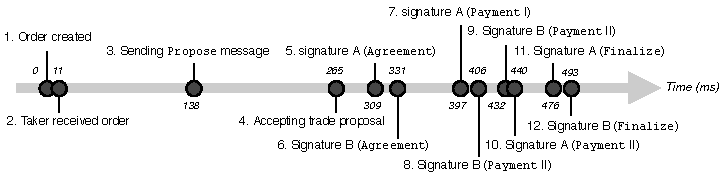
\includegraphics[width=\linewidth]{xchange/assets/trade_timeline}
	\caption{A timeline of the events during a single trade between a maker $ A $ and a taker $ B $. The experiment is conducted on two hosted Raspberry Pis (3rd generation, model B+). The total duration of the trade is 493 milliseconds.}
	\label{fig:trade_timeline}
\end{figure}

\textbf{Results.}
Figure \ref{fig:trade_timeline} shows a timeline of the events during a single trade between the two Raspberry Pis.
The full trade sequence, from the moment of order creation to mutual possession of a dual-signed \texttt{Finalize} transaction, completes in 493 milliseconds, less than half a second.
Almost half of the trade duration, 254 milliseconds, is spent in phase II of the \ModelName{} trading protocol, the trade negotiation phase.
During this phase, a trader determines whether a counterparty is already involved in a trade by inspection of the records in the TrustChain ledger of the other party.

\textbf{Conclusion.}
This experiment shows that a full trade, including order creation, can be completed within half a second on low-resource devices if asset transfer would be instant.
Based on this experiment, we argue that the deployment of \ModelName{} in an Internet-of-Things (IoT) environment would be viable since its communication and transaction creation overhead is minimal.
Asset management is a common feature in IoT~\cite{gilchrist2016industry}.
\ModelName{} can be used to coordinate asset exchange between different IoT environments.
However, our trading protocol requires periodic inspection of blockchain during an ongoing trade.
Since maintaining a full transaction history is not realistic given the storage restrictions of IoT devices, \ModelName{} should rely on dedicated full nodes that have to appropriate credentials to participate in a specific blockchain.
We believe that devices with less processing capabilities than Raspberry Pis are still capable of maintaining and securing TrustChain records.
This belief should be verified with further experimentation through a small-scale deployment of \ModelName{} in an IoT environment where blockchain-based assets are managed and traded.

Even though the low trade duration on low-resource devices is a promising result, the experiment is not representative of a realistic trading environment where there are many traders creating orders and exchanging assets simultaneously.
Furthermore, the prior experiment does not reveal the impact of our risk mitigation strategies on performance.
Therefore, our next experiment focuses on the scalability of \ModelName{} and shows how our mechanism behaves under a higher system load.

\subsection{Scalability of \ModelName{}}
\label{subsec:scalability_experiment}
We now perform scalability experiments to quantify the performance of \ModelName{} as the system load and network size increases.

\textbf{Setup.}
To explore the limitations and overhead of \ModelName{}, we conduct scalability experiments on our university cluster.
The detailed specifications of the hardware and runtime environment can be found online.\footnote{https://www.cs.vu.nl/das5/}
Our infrastructure allows us to reserve computing nodes and deploy instances of \ModelName{} on each node.
We use the Gumby experiment framework to orchestrate the deployment of \ModelName{} instances onto computing nodes and to extract results from experiment artifacts.\footnote{https://github.com/tribler/gumby}
The scalability experiment is controlled by a \emph{scenario file}, a chronologically ordered list of actions which are executed by all or by a subset of running instances, at specific points in time after the experiment starts.
Each run is performed at least five times, and the results are averaged.

We increase the system load, namely the number of new orders being created every second.
As the system load grows, so does the number of traders in the network.
We devise a synthetic dataset to determine the performance of \ModelName{} under a predictable arrival rate of orders.
In a network with $ n $ peers running \ModelName{}, $ n $ orders are created every half a second.
To avoid the situation where all instances create new orders at the same time, the starting time of this periodic order creation is uniformly distributed over all peers, based on their assigned IDs (ranging from 1 to $ n $).
Each peer acts as a matchmaker and sends a new order to four matchmakers, which each peer randomly selects when the experiment starts.
The experiment lasts for 30 seconds, after which $ 30n $ orders are created in total.
Each order buys a single token in return for another token, to make matchmaking a predictable process.
After 30 seconds, the experiment is terminated.

We test the scalability of \ModelName{} under a combination of the two risk mitigation strategies discussed in Section~\ref{sec:solution_outline}.
With the $ INC\_SET(n) $ policy, we refer to the incremental settlement strategy where each trader makes $ n $ payments to the counterparty during a single trade.
The $ RESTRICT $ policy denotes the policy where a trader follows the \ModelName{} rules to verify whether it should trade with another party or not (see Section \ref{sec:limit_risk}).
We consider four experiment settings in total, with combinations of the $ RESTRICT $ and $ INC\_SET(2) $ policies, and when no risk mitigation policy is active.
Scalability is measured as follows:
first, we analyze the peak \emph{throughput} observed during the experiment, in terms of trades per second.
Second, we consider the average order fulfill \emph{latency}, which is the time between the creation of an order and the time until this order has been completed (the order creator has exchanged all assets as specified in the order).

\begin{figure*}[t]
	\centering
	\begin{subfigure}[t]{.5\textwidth}
		\centering
		\captionsetup{width=.9\linewidth}
		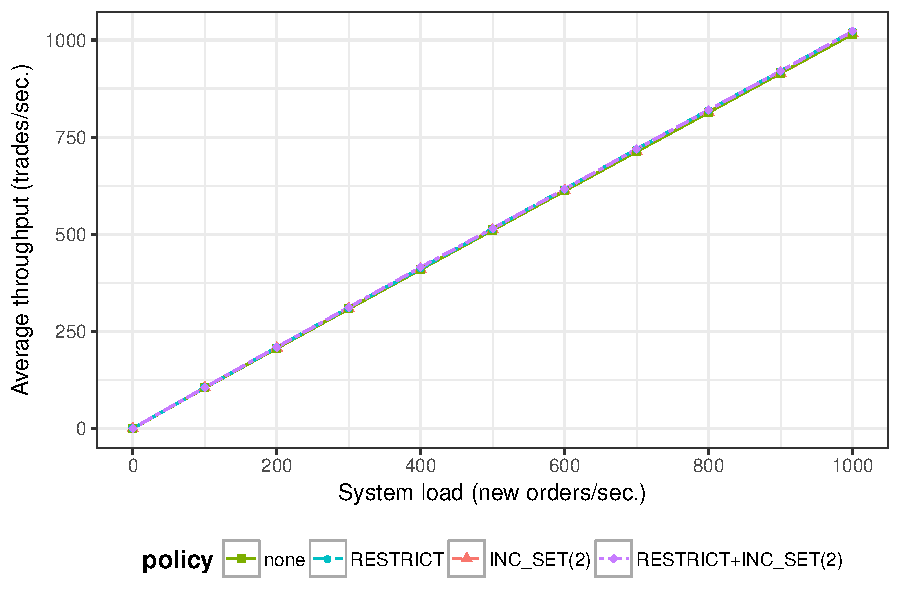
\includegraphics[width=.95\linewidth]{xchange/assets/experiments/scalability}
		\caption{Peak throughput}
		\label{fig:scalability}
	\end{subfigure}%
	\begin{subfigure}[t]{.5\textwidth}
		\centering
		\captionsetup{width=.9\linewidth}
		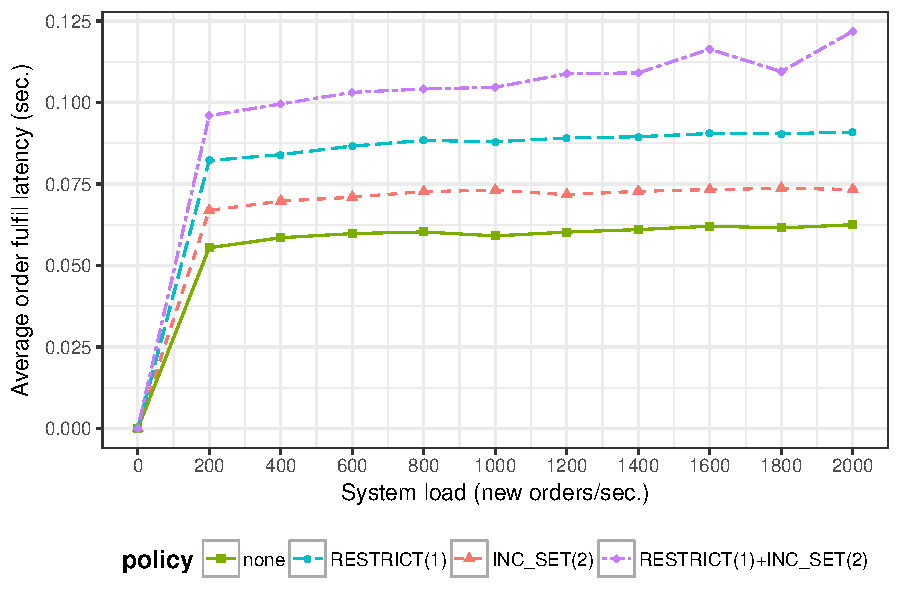
\includegraphics[width=.95\linewidth]{xchange/assets/experiments/latency}
		\caption{Average order fulfill latency}
		\label{fig:latency}
	\end{subfigure}%
	\caption{The peak throughput and order fulfill latencies as the system load increases.}
	\label{fig:scalability_latency}
\end{figure*}

\textbf{Results.}
The results of the scalability experiments are presented in Figure~\ref{fig:scalability_latency}.
We run each experiment with a specific system load up to 1.000 deployed instances (which is close to the limitations of the used hardware).
Figure~\ref{fig:scalability} shows how the peak throughput (expressed in trades per second, vertical axis) behaves with respect to the system load (horizontal axis).
All experiment settings hint at linear scalability as the system load increases.
Furthermore, enabling risk mitigation policies does not appear to have a notable effect on the peak throughput.
Experimentation on more compute nodes should reveal whether this trend continues when the system load exceeds 1.000 new orders per second.

Figure~\ref{fig:latency} shows the average order fulfill latency when the system load increases, for the four evaluated experiment settings.
The average order fulfill latency remains largely constant when the system load grows.
Applying the restriction and incremental settlement policies increases the average order fulfill latency, since more operations have to be performed to successfully complete an order.
We observe a moderate increase of latency when applying the $ RESTRICT + INC_SET (2) $ policies when the system load grows to 1.000 trades per second.
The high system load is likely to increase the duration of individual trades beyond 0.5 seconds, which means that the $ RESTRICT $ policy prevents traders from initiating a new trade with others.
Since a trader now has to find a new party to trade with, the average order fulfill latency increases.

\textbf{Conclusion.}
The main finding of this experiment is that the throughput (trades per second) scales linearly with respect to the system load and network size.
We also observe that the average order fulfill latency remains largely constant as the system load grows.
Further experimentation should reveal whether these trends continue with an even higher system load.

\section{Conclusions}
We have presented \ModelName{}, a universal mechanism for asset exchange between permissioned blockchain.
\ModelName{} facilitates asset exchange without relying on particular transaction types or trusted third parties to mediate in the trading process.
\ModelName{} records the initiation of a trade, individual payments, and the completion of a trade in a distributed log.
By devising a set of rules that define when a party should engage in a new trade, we have limited the economic gains of adversarial parties.
Specifically, when an adversary commits counterparty fraud, any further trade with this adversary are refused by honest parties until the fraud is resolved.
Incremental settlement further reduces economic gains by splitting each payment into multiple, smaller ones.

With an open-source implementation and an experimental evaluation, we have demonstrated the viability of trading on devices with low hardware capabilities.
A single trade can be completed within half a second if asset transfers on external blockchain platforms would finish instantly.
With a scalability experiment on our compute cluster, we achieved over 1.000 trades per second and found that the throughput of \ModelName{} in terms of trades per second scales linearly with the system load and network size.
